\documentclass[]{beamer}
%\documentclass[handout]{beamer}
\usetheme{Boadilla} 
%\usecolortheme{seagull}
%\setbeamerfont*{frametitle}{size=\normalsize,series=\bfseries}
%\setbeamertemplate{blocks}[default]%[shadow=false]

\setbeamertemplate{footnote}{\tiny\makebox[1em][l]{\insertfootnotemark}\insertfootnotetext\par}



%\setbeamertemplate{footnote}{\hangpara{1em}{1}\makebox[1em][l]{\insertfootnotemark}\scriptsize\insertfootnotetext\par}

%\definecolor{icml_tutorial}{RGB}{181,74,16}

%\setbeamercolor{title}{bg=icml_tutorial,fg=white}

%\usetheme{Boadilla}
\usefonttheme{professionalfonts}
%%\usecolortheme{seagull}
\usefonttheme[onlymath]{serif}
%
\setbeamertemplate{blocks}[rounded][shadow=false]

\usepackage{array}
%\usepackage{algorithm}
%\usepackage{algorithmic}
%\usepackage[english]{babel}
\usepackage{booktabs} 
\usepackage{graphicx}
\usepackage{amssymb}
\usepackage{amsmath}
\usepackage{stmaryrd} 
\usepackage{dsfont}
\usepackage{color,colortbl} 
\usepackage{pgfplots}
%\usepackage{bibentry}
\usepackage{algorithm}
\usepackage[noend]{algpseudocode}
\usepackage{tikz}
\usetikzlibrary{mindmap,trees}
\usetikzlibrary{decorations.pathreplacing}
\usetikzlibrary{decorations.pathmorphing}
\usetikzlibrary{arrows}
\usetikzlibrary{positioning}
\usetikzlibrary{decorations.text}
\usetikzlibrary{decorations.markings}
\usetikzlibrary{decorations.shapes}
\usetikzlibrary{shapes,snakes}
\usetikzlibrary{calc,trees,positioning,arrows,chains,shapes.geometric,
  decorations.pathreplacing,decorations.pathmorphing,shapes,matrix,shapes.symbols}
\usetikzlibrary{shapes.misc}

\usepackage{multirow}
% \usepackage{beamerthemesplit} // Activate for custom appearance



 
\newcommand{\lsize}{m}
\newcommand{\osize}{n}
\newcommand{\qsize}{q}
\newcommand{\odsize}{d}
\newcommand{\qdsize}{r}
\newcommand{\ispace}{\mathcal{X}}
\newcommand{\taskspace}{\mathcal{T}}
\newcommand{\objspace}{\mathcal{D}}
\newcommand{\anyspace}{\mathcal{X}}
\newcommand{\hypspace}{\mathcal{H}}
\newcommand{\kernelf}{k}
\newcommand{\gkernelf}{g}
\newcommand{\kkernelf}{\Gamma}
\newcommand{\dkernelm}{\bm{K}}
\newcommand{\tkernelm}{\bm{G}}
\newcommand{\kkernelm}{\bm{\Gamma}}
\newcommand{\regparam}{\lambda}
\newcommand{\idmatrix}{\bm{I}}
\newcommand{\trace}{\textnormal{tr}}
%\newcommand{\transpose}{^\textnormal{T}}
\newcommand{\transpose}{^\intercal}
\newcommand{\bm}[1]{\mathbf{#1}}
\newcommand{\ve}{\textnormal{vec}}
\newcommand{\mat}{\textnormal{mat}}
\newcommand{\diagv}{\textnormal{diag}_v}
\newcommand{\diagm}{\textnormal{diag}_m}
\newcommand{\LOO}{\text{LOO}}
\newcommand{\predfun}{f}
\newcommand{\filterfun}{\varphi}
\newcommand{\objset}{D}
\newcommand{\taskset}{T}
\newcommand{\labelvec}{\bm{y}}
\newcommand{\Algo}[1]{{#1}}


\setbeamertemplate{footline}[frame number]
\beamertemplatenavigationsymbolsempty 
%\logo{
\includegraphics[height=1.2cm]{Figures/Kermit}}



\renewcommand{\Pr}{P}
\newcommand{\cumPr}{\mathbf{P}}
\renewcommand{\vec}[1]{\boldsymbol{#1}}
\newcommand{\brY}{\vec{Y}}
\newcommand{\given}{\, | \,}
\newcommand{\cumprob}{P}
\newcommand{\cumprobx}{P_{\vec{x}}}
\newcommand{\probx}{p_{\vec{x}}}
\newcommand{\probxi}[1]{p_{\vec{x}}^{(#1)}}
\newcommand{\invmarg}[1]{P_{\vec{x},#1}^{-1}}
\newcommand{\cop}{C}
\newcommand{\dcop}{c}
\newcommand{\copx}{C_{\vec{x}}}
\newcommand{\dcopx}{c_{\vec{x}}}
\newcommand{\mx}[1]{\mathbf{\mathrm{#1}}}
\newcommand{\maxprobxi}[1]{p_{\vec{x},max}^{(#1)}}
\newcommand{\minprobxi}[1]{p_{\vec{x},min}^{(#1)}}
\DeclareMathOperator*{\argmax}{\arg \max}
\DeclareMathOperator*{\argmin}{\arg \min}

\newcommand{\Fb}{F}
\newcommand{\loss}{L}
\newcommand{\ells}{\tilde{\ell}}
\newcommand{\regret}{\textnormal{Reg}}
\newcommand{\lossrank}{L_{\textnormal{\scriptsize{rnk}}}}
\newcommand{\ellrank}{\ell_{\textnormal{\scriptsize{rnk}}}}
\newcommand{\regretrank}{{\textnormal{Reg}}_{\textnormal{\scriptsize{rnk}}}}
%\newcommand{\lossranktilde}{L_{\widetilde{rnk}}}
%\newcommand{\regretranktilde}{{\textnormal{Reg}}_{\widetilde{rnk}}}
\newcommand{\lossranktilde}{\lossrank}
\newcommand{\regretranktilde}{\regretrank}
\newcommand{\lossexp}{L_{\textnormal{\scriptsize{exp}}}}
\newcommand{\ellexp}{\ells_{\textnormal{\scriptsize{exp}}}}
\newcommand{\regretexp}{{\textnormal{Reg}}_{\textnormal{\scriptsize{exp}}}}
\newcommand{\losslog}{L_{\textnormal{\scriptsize{log}}}}
\newcommand{\elllog}{\ells_{\textnormal{\scriptsize{log}}}}
\newcommand{\regretlog}{{\textnormal{Reg}}_{\textnormal{\scriptsize{log}}}}
\newcommand{\lossrankbar}{L_{\textnormal{\scriptsize{br}}}}
\newcommand{\ellrankbar}{\ell_{\textnormal{\scriptsize{br}}}}
\newcommand{\regretrankbar}{{\textnormal{Reg}}_{\textnormal{\scriptsize{br}}}}

\newcommand{\sgn}[1]{\textrm{sgn}\left(#1\right)}
%\newcommand{\bm}{\mathds{1}}
\newcommand{\ZO}{0/1 }
\newcommand{\bx}{\boldsymbol{x}}
\newcommand{\by}{\boldsymbol{y}}
\newcommand{\bh}{\boldsymbol{h}}
\newcommand{\bY}{\boldsymbol{Y}}
\newcommand{\bX}{\boldsymbol{X}}
\newcommand{\bz}{\boldsymbol{z}}
%\newcommand{\bm}{\mathds{1}}
\newcommand{\assert}[1]{\llbracket #1 \rrbracket}
%\newcommand{\assert}[1]{\bm [ #1 ] } %[\llbracket #1 \rrbracket}
\newcommand{\colorcell}{\multicolumn{1}{>{\columncolor{DarkGreen}}l}{}}
\newcommand{\graytextcell}[1]{\begin{color}{gray}#1\end{color}}
\newcommand{\calX}{\mathcal{X}}
\newcommand{\calY}{\mathcal{Y}}
\newcommand{\calH}{\mathcal{H}}
\newcommand{\calL}{\mathcal{L}}
\newcommand{\calO}{\mathcal{O}} 
\newcommand{\calC}{\mathcal{C}} 

%\newcommand{\loss}{L}
%\newcommand{\regret}{\textnormal{Reg}}
\newcommand{\lossell}{L_{\ell}}
\newcommand{\regretell}{\textnormal{Reg}_{\ell}}
%\newcommand{\lossrank}{L_{\textnormal{\scriptsize{rank}}}}
%\newcommand{\regretrank}{{\textnormal{Reg}}_{\textnormal{\scriptsize{rank}}}}
%\newcommand{\sgn}[1]{\textrm{sgn}\left(#1\right)}
%\newcommand{\bm}{\mathds{1}}

\definecolor{putblue}{RGB}{0,0,124}
\definecolor{putred}{RGB}{204,33,69}
\renewcommand{\alert}[1]{\textbf{\color{putblue} #1}}
\renewcommand{\emph}[1]{\textbf{\color{putblue}#1}}
%\renewcommand{\emph}[1]{\textbf{\color{icml_tutorial}#1}}


\setbeamercolor{title}{bg=white,fg=putblue}
\setbeamercolor{subtitle}{bg=white,fg=putblue}

%\newcommand {\autographics}[1] {
  %\begin{center}
    %\includegraphics[width=\textwidth,height=0.85\textheight,keepaspectratio]{#1}
  %\end{center}
%}
%\newcommand {\autographicswithsize}[2] {
  %\begin{center}
    %\includegraphics[width=\textwidth,height=#2\textheight,keepaspectratio]{#1} 
  %\end{center}
%}

%\newcommand {\autographicswithsizew}[2] {
  %\begin{center}
  %\vskip-20pt
    %\includegraphics[width=\textwidth,width=#2\textheight,keepaspectratio]{#1}
  %\vskip5pt
  %\end{center}
%}

%\def\newblock{\hskip .11em } %plus .33em minus .07em}


\title[]{Multi-Target Prediction:\\ 
A Unifying View on Problems and Methods}
\author[Willem Waegeman]{Willem Waegeman and Dimitrios Iliadis} 
%\author[Eyke]{Eyke H\"ullermeier}
%\date[NIPS 2015]{NIPS: extreme classification workshop\\December 12, 2015}
\institute[VFU] % (optional)
{
  \inst{}
Department of Data Analysis and Mathematical Modelling, Ghent University, Belgium
}

%\date{Winter School on Machine Learning, Gran Canaria, 2020 }

\begin{document}

\frame{\titlepage}


\section{Introduction}

%\begin{frame}[plain]
        %\begin{tikzpicture}[remember picture,overlay]
            %\node[at=(current page.center)] {
                %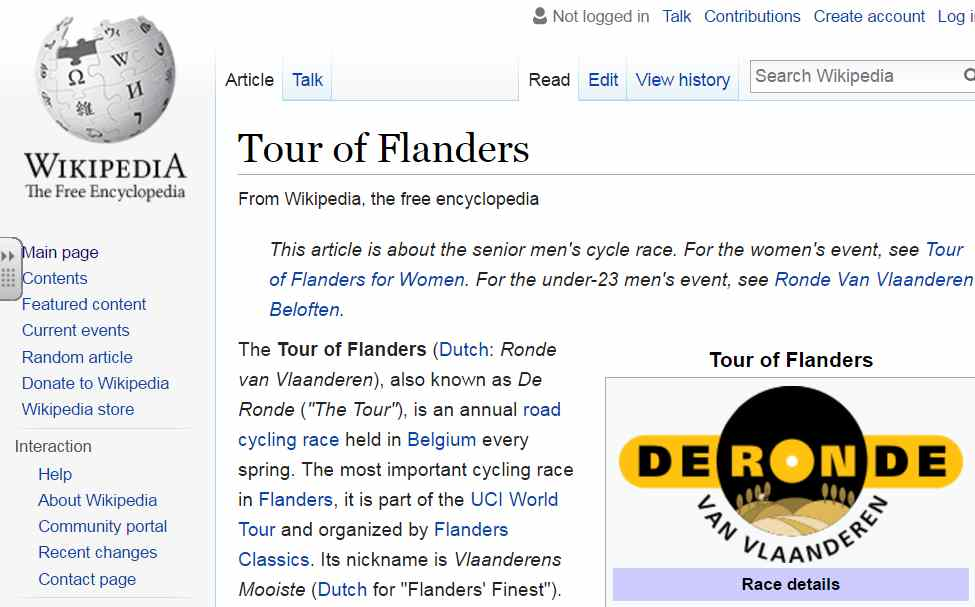
\includegraphics[scale=0.35]{pics/flanders}
            %};
        %\end{tikzpicture}
     %\end{frame}
		
		\begin{frame}[plain]
        \begin{tikzpicture}[remember picture,overlay]
            \node[at=(current page.center)] {
                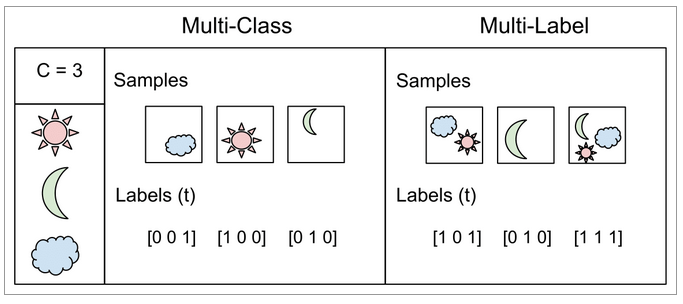
\includegraphics[scale=0.5]{pics/multi-classlabel}
            };
        \end{tikzpicture}
     \end{frame}

%\section{Introduction}


\begin{frame}{Multi-label classification: \\
the example of document categorization}
% voorbeeldje met boeken
\includegraphics[scale=0.17]{pics/kompany}
\end{frame}

\begin{frame}{Multi-label classification: \\
the example of document categorization}
% voorbeeldje met boeken
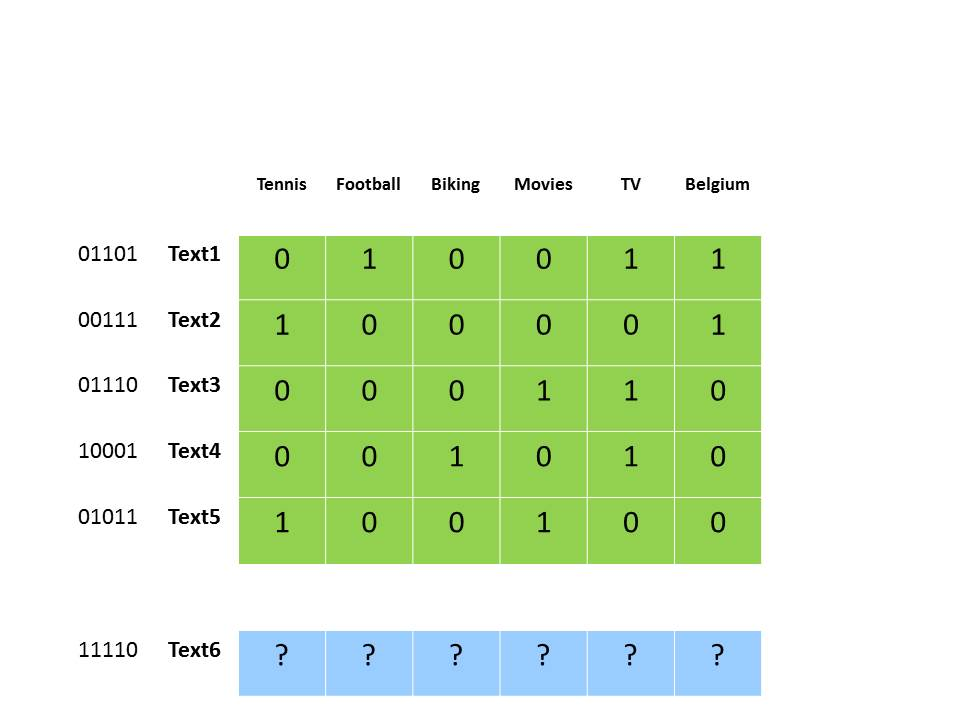
\includegraphics[width=0.9\textwidth,trim = 0 0 100 100,clip]{Figures/pictures/Slide2}
\end{frame}

\begin{frame}[plain]
        \begin{tikzpicture}[remember picture,overlay]
            \node[at=(current page.center)] {
                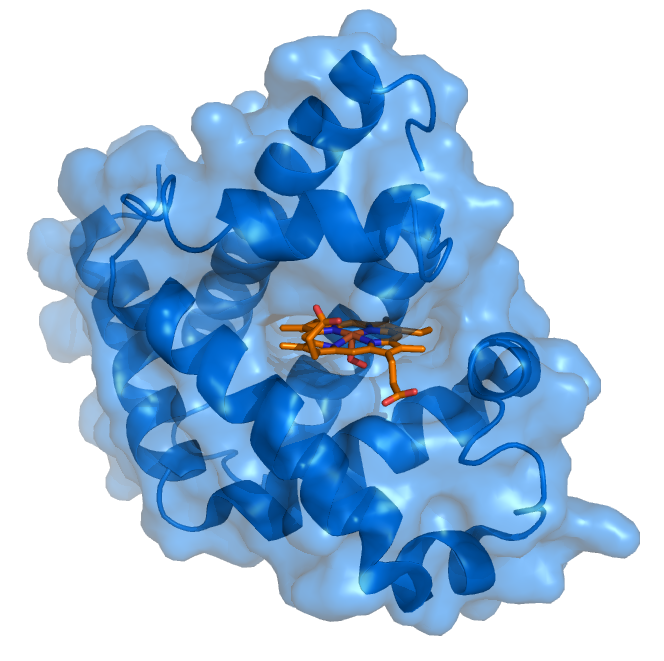
\includegraphics[width=0.7\textwidth]{pics/proteinl}
            };
        \end{tikzpicture}
     \end{frame}

\begin{frame}{Multivariate regression: \\
the example of protein-ligand interaction prediction}
% voorbeeldje met boeken
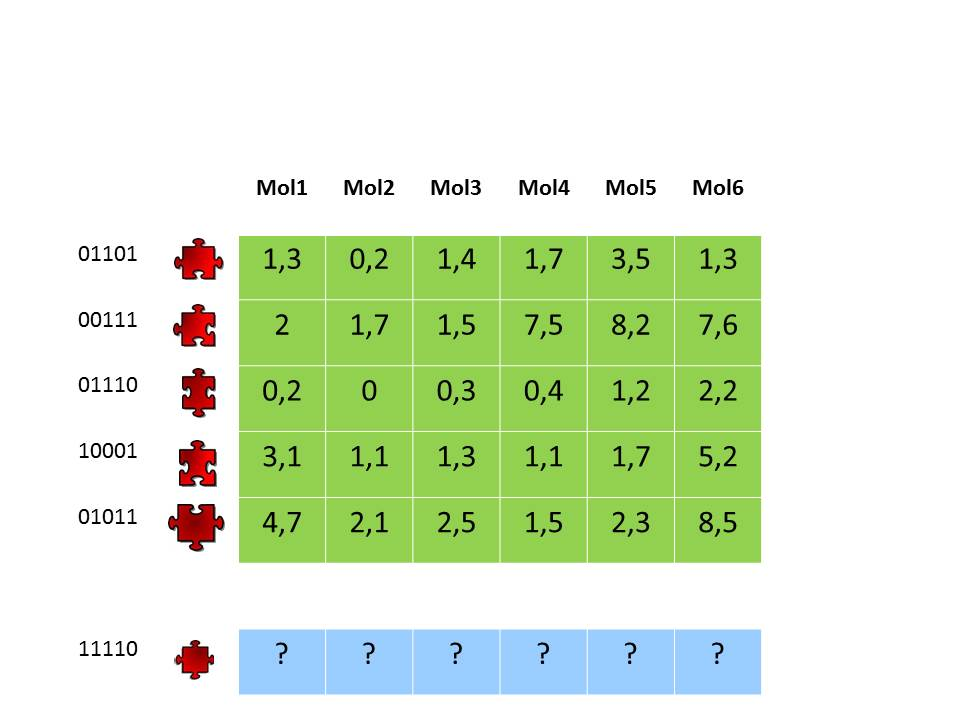
\includegraphics[width=0.9\textwidth,trim = 0 0 100 100,clip]{Figures/pictures/Slide1}
\end{frame}

\begin{frame}[plain]
        \begin{tikzpicture}[remember picture,overlay]
            \node[at=(current page.center)] {
                
\includegraphics[width=\textwidth]{Figures/school_shopping}
            };
        \end{tikzpicture}
     \end{frame}

\begin{frame}{Multi-task learning: \\
the example of predicting student marks}
% voorbeeldje met boeken
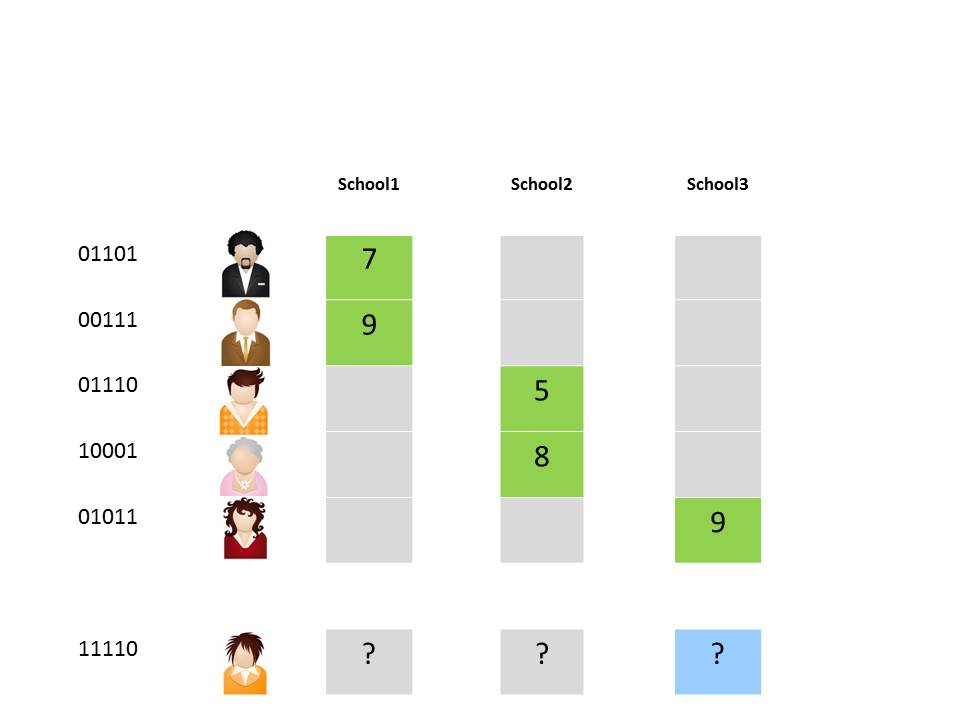
\includegraphics[width=0.9\textwidth,trim = 0 0 100 100,clip]{Figures/pictures/Slide3}
\end{frame}



%\begin{frame}{Other cool applications: ecology}
   %\center 
   %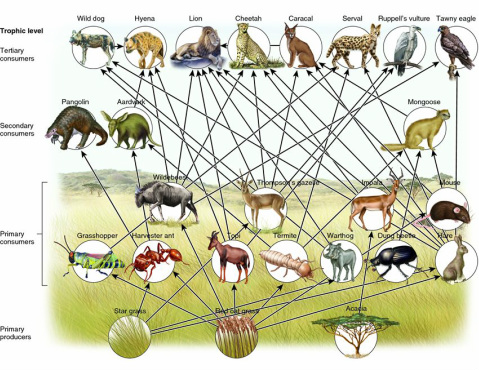
\includegraphics[width=10cm]{Figures/foodweb.jpg}
   %\vfill
   %%Predicting links between \alert{people}
 %% social network prediction, protein ligand prediction, food pairing, image analysis: voorbeeld?
%\end{frame}

%\begin{frame}{Other cool applications: food pairing}
   %\center 
   %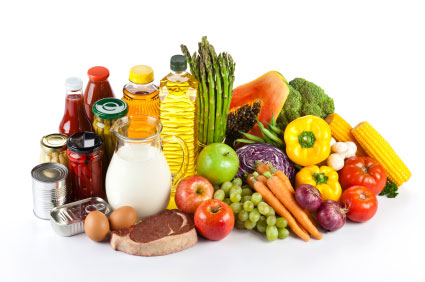
\includegraphics[width=\textwidth]{Figures/ingredients}
   %\vfill
 %% social network prediction, protein ligand prediction, food pairing, image analysis: voorbeeld?
%\end{frame}

%
%\begin{frame}{The two-step ridge regression}
%Prediction function:
%
%$$
%f(d, t) = \boldsymbol{\phi}(d)^\intercal\mathbf{W}  \boldsymbol{\psi}  (t) 
%$$
%
%Parameters can be found by solving:
%$$
%\boldsymbol{\Phi}^\intercal\mathbf{Y}\boldsymbol{\Psi} = (\boldsymbol{\Phi}^\intercal\boldsymbol{\Phi}+\lambda_d\mathbf{I})\mathbf{W}(\boldsymbol{\Psi}^\intercal\boldsymbol{\Psi}+\lambda_t\mathbf{I})
%$$
%\pause
%Two hyperparameters: $\lambda_d$ and $\lambda_t$!
%\end{frame}

\begin{frame}{There are a lot of multi-target prediction problems around...}

\begin{center}
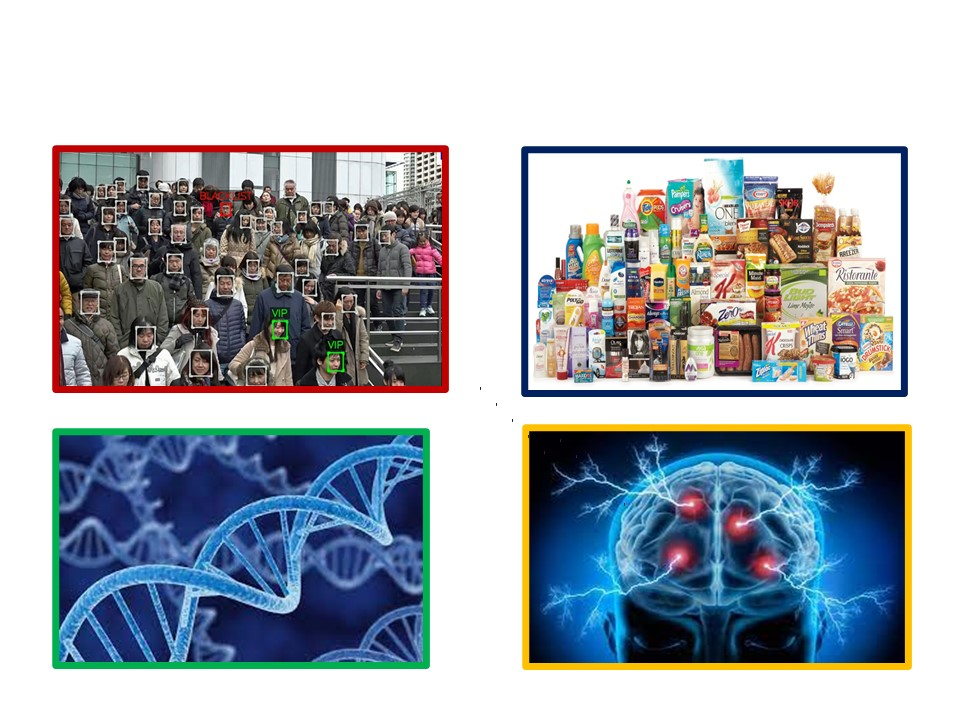
\includegraphics[width=\textwidth,trim = 0 0 0 70,clip]{Figures/pictures/Slide25}
\end{center}

\end{frame} 

\begin{frame}{Matrix completion: a recommender system}

\begin{center}
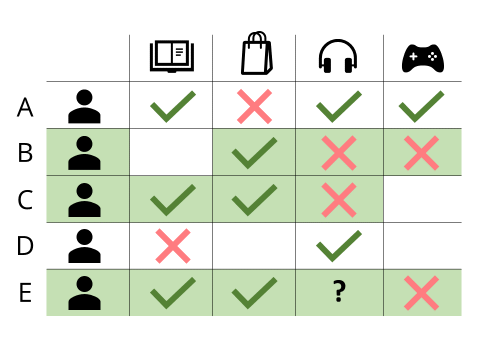
\includegraphics[scale=0.5]{Figures/collafilt}
\end{center}

\end{frame}

\begin{frame}{Matrix completion: a genomics example}

\begin{center}
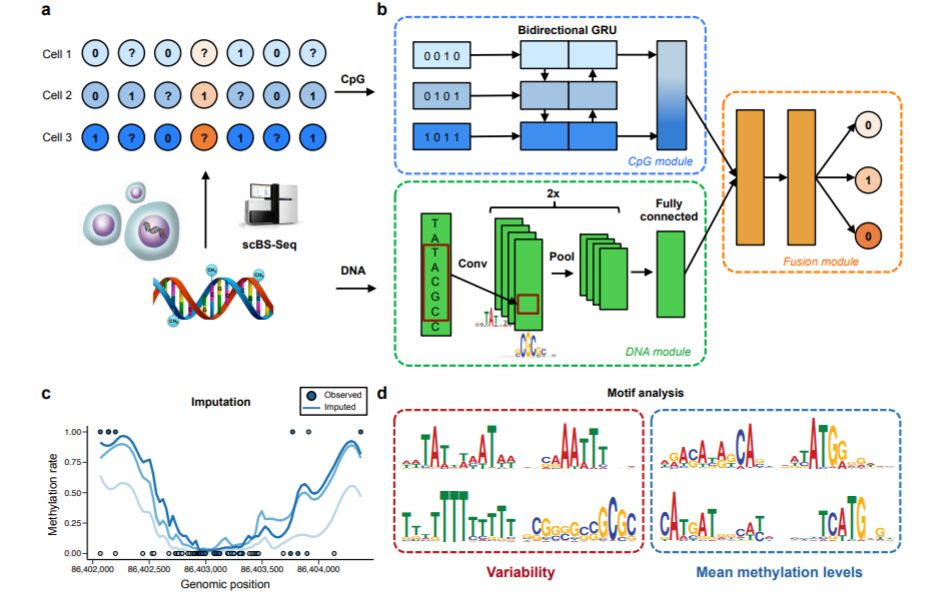
\includegraphics[scale=0.3]{Figures/deepcpg} \\
Angermueller et al.\ Accurate prediction of single-cell DNA methylation states
using deep learning, Genome Biology, 2017.

\end{center}

\end{frame}

\begin{frame}{Multi-task learning: detecting epileptic seizures}
% voorbeeldje met boeken
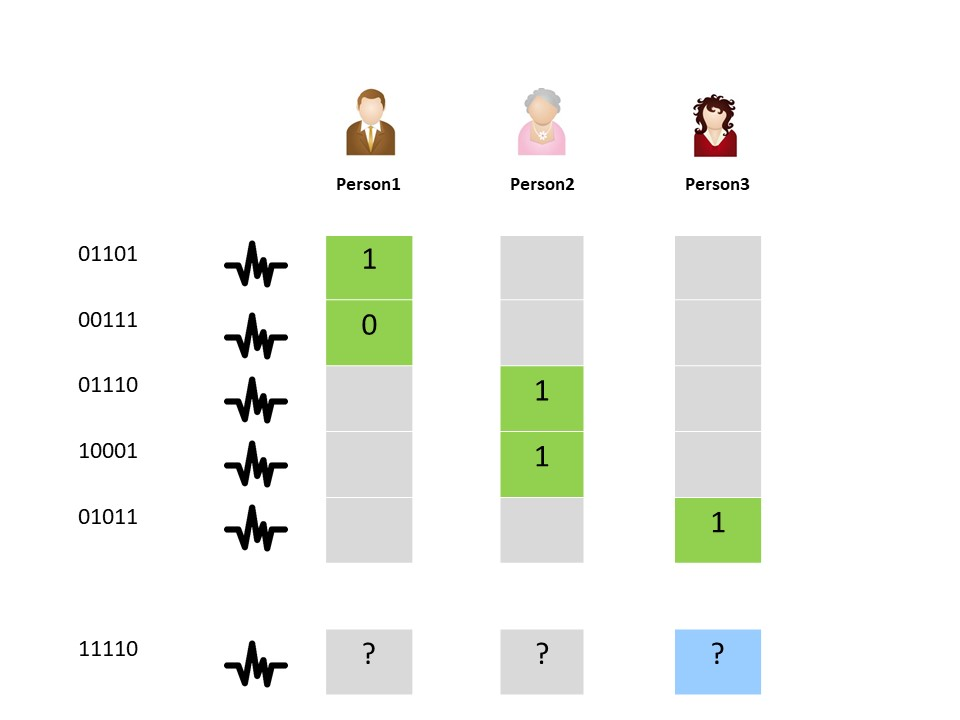
\includegraphics[width=0.9\textwidth,trim = 0 0 100 50,clip]{Figures/pictures/Slide24}
\end{frame}


\begin{frame}{Accompanying article}

\begin{center}
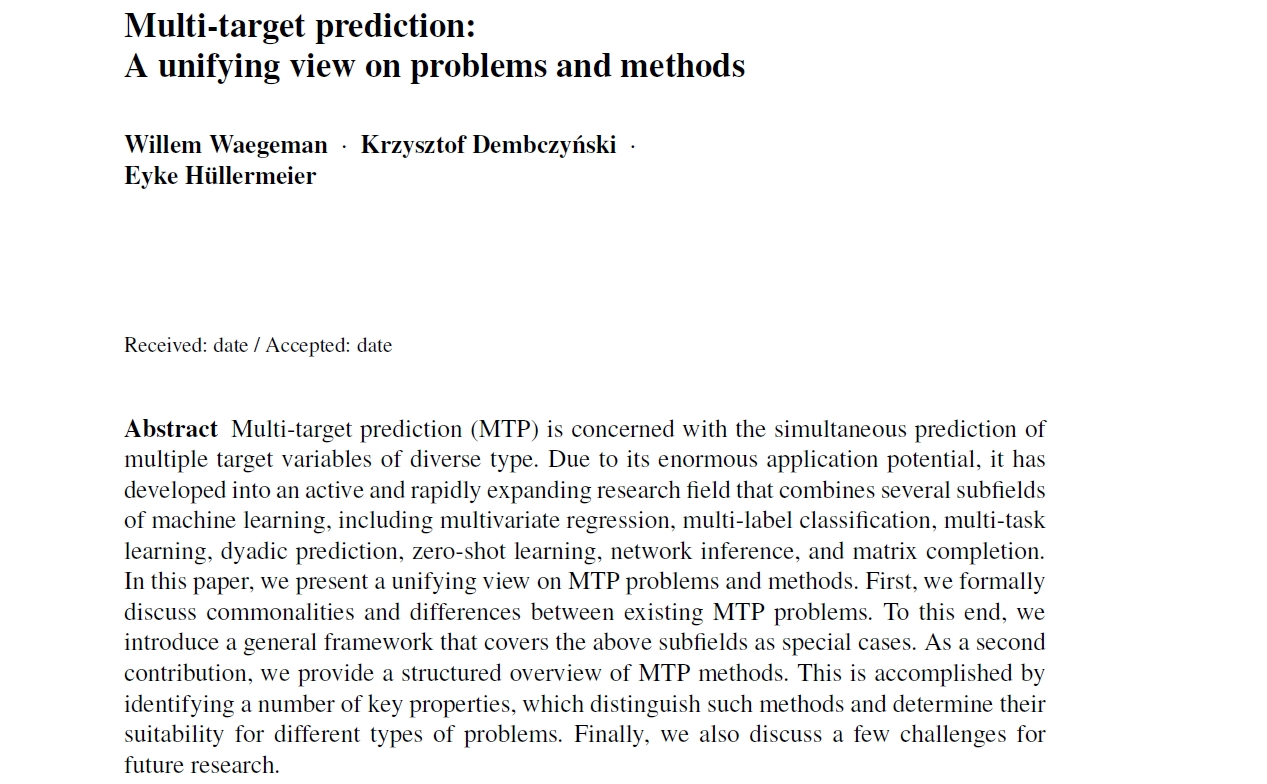
\includegraphics[width=\textwidth,trim = 0 0 0 0,clip]{Figures/dami}\\
Data Mining and Knowledge discovery, 2019. 
\end{center}

\end{frame}


%%% begin changes %%%


\section{A unifying view on MTP problems}


\begin{frame}{Overview of this talk}

\tableofcontents

\end{frame}




%\begin{frame}
%\frametitle{Multi-target prediction}
%\begin{itemize}
%\item \emph{Multi-Target Prediction:} For a feature vector $\bx$ predict accurately \\a vector of responses $\by$ using a function $\bh(\bx)$:
%$$
%\bx = (x_1,x_2,\ldots,x_p) \xrightarrow{~~\bh(\bx)~~} \by = (y_1, y_2, \ldots, y_m)
%$$
%\item \emph{Main challenges:} 
%\begin{itemize}
%\item Appropriate modeling of target dependencies between targets 
%$$
%y_1, y_2, \ldots, y_m
%$$
%\item A multitude of multivariate loss functions defined over the output vector 
%$$\ell(\by, \bh(\bx))$$
%%to measure the quality of prediction.
%\end{itemize}
%\item \emph{Main question:} %Can we improve over independent models trained for each target?
%\begin{itemize}
%\item Can we improve over independent models trained for each target? 
%\end{itemize}
%\item \emph{Two views:} %the individual target and joint target view.
%\begin{itemize}
%\item The individual-target view
%\item The joint-target view
%\end{itemize}
%\end{itemize}
%
%\end{frame}

\begin{frame}{General framework}
\begin{definition}
A multi-target prediction setting is characterized by instances $\vec{x} \in \mathcal{X}$ and targets $\vec{t} \in \mathcal{T}$ with the following properties: 
\begin{itemize} 
\item[1.] A training dataset consists of triplets $(\vec{x}_i,\vec{t}_j,y_{ij})$, where $y_{ij} \in \mathcal{Y}$.  
\item[2.] In total $n$ instances and $m$ targets are observed during training, with $n$ and $m$ finite numbers. 
\item[3.]As such, the scores $y_{ij}$ of the training data can be arranged in an $n \times m$ matrix $Y$.
\item[4.] The score set $\mathcal{Y}$ is one-dimensional. It consists of nominal, ordinal or real values.  
\item[5.] The goal consists of making predictions for any instance-target couple $(\vec{x},\vec{t}) \in \mathcal{X} \times \mathcal{T}$.   
\end{itemize}
\end{definition}
\end{frame}

\begin{frame}{Conventional MTP settings}
\begin{itemize}
\item Side information for targets is normally not available. 
\item \emph{Multi-label classification} (e.g., assigning appropriate category tags to documents).
\item \emph{Multivariate regression} (e.g., predicting whether a protein will bind to a set of experimentally developed small molecules).
\item \emph{Multi-task learning} (e.g., predicting student marks in the final exam for a typical high-school course).
\end{itemize}
\end{frame}





\begin{frame}{Conventional MTP settings}
\begin{definition}[Multi-label classification] 
A multi-label classification problem is a specific instantiation of the general framework, which exhibits the following additional properties: 
\begin{enumerate}
\item[P5.] The cardinality of $\mathcal{T}$ is $m$; this implies that all targets are observed during training. 
\item[P6.] No side information is available for targets. Again, without loss of generality, we can hence identify targets with natural numbers, such that the target space is $\mathcal{T} = \{1,...,m\}$. 
\item[P7.] The score matrix $Y$ has no missing values. 
\item[P8b.] The score set is $\mathcal{Y} = \{0,1\}$. 
\end{enumerate}
\end{definition}
\end{frame}

\begin{frame}{Multi-label classification}
% voorbeeldje met boeken
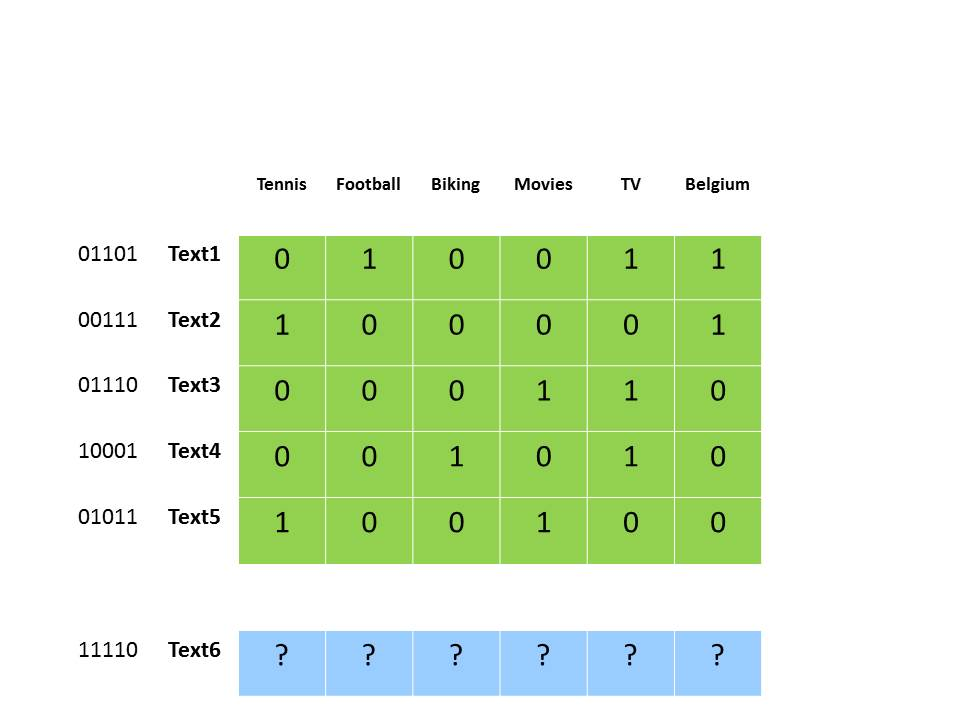
\includegraphics[width=0.9\textwidth,trim = 0 0 100 100,clip]{Figures/pictures/Slide2}
\end{frame}

\begin{frame}{Conventional MTP settings}
\begin{definition}[Multivariate regression] 
A multivariate regression problem is a specific instantiation of the general framework, which exhibits the following additional properties: 
\begin{enumerate}
\item[P5.] The cardinality of $\mathcal{T}$ is $m$. This implies that all targets are observed during training. 
\item[P6.] No side information is available for targets. Without loss of generality, we can hence assign the numbers $1$ to $m$ as identifiers to targets, such that the target space is $\mathcal{T} = \{1,...,m\}$. 
\item[P7.] The score matrix $Y$ has no missing values. 
\item[P8.] The score set is $\mathcal{Y} = \mathbb{R}$. 
\end{enumerate}
\end{definition}
\end{frame}

\begin{frame}{Multivariate regression}
% voorbeeldje met boeken
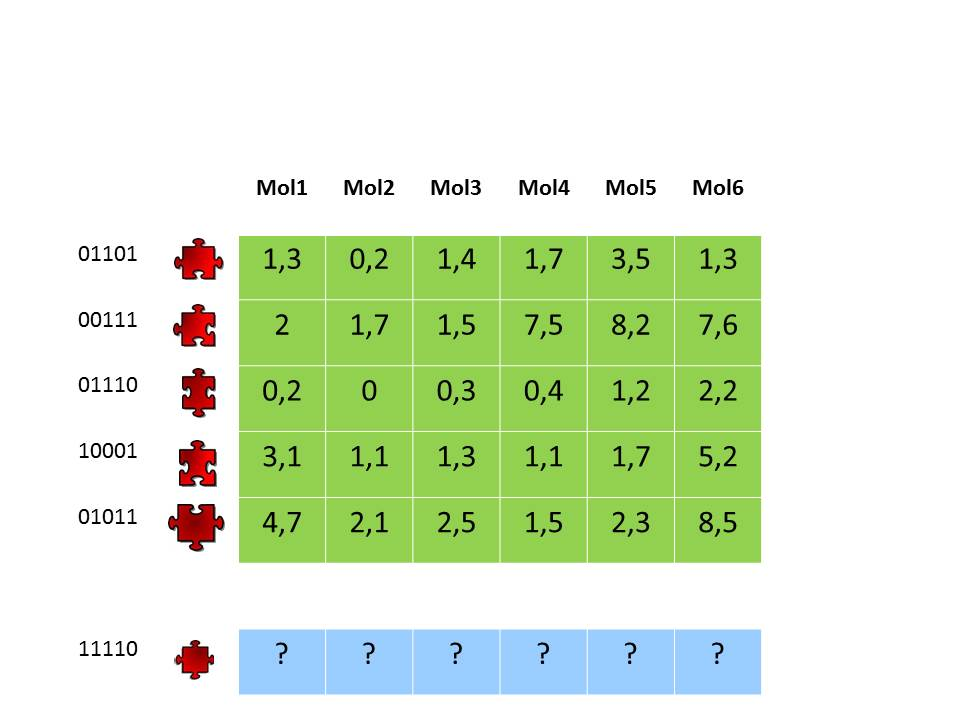
\includegraphics[width=0.9\textwidth,trim = 0 0 100 100,clip]{Figures/pictures/Slide1}
\end{frame}

\begin{frame}{Conventional MTP settings}
\begin{definition}[Multi-task learning] 
A multi-task learning problem is a specific instantiation of the general framework, which exhibits the following additional properties: 
\begin{enumerate}
\item[P5.] The cardinality of $\mathcal{T}$ is $m$; this implies that all targets are observed during training. 
\item[P6.] No side information is available for targets. Again, the target space can hence be taken as $\mathcal{T} = \{1,...,m\}$.   
\item[P8a.] The score set is homogenous across columns of $Y$, e.g., $\mathcal{Y} = \{0,1\}$ or $\mathcal{Y} = \mathbb{R}$.
\end{enumerate}
\end{definition}
\end{frame}


\begin{frame}{Multi-task learning}
% voorbeeldje met boeken
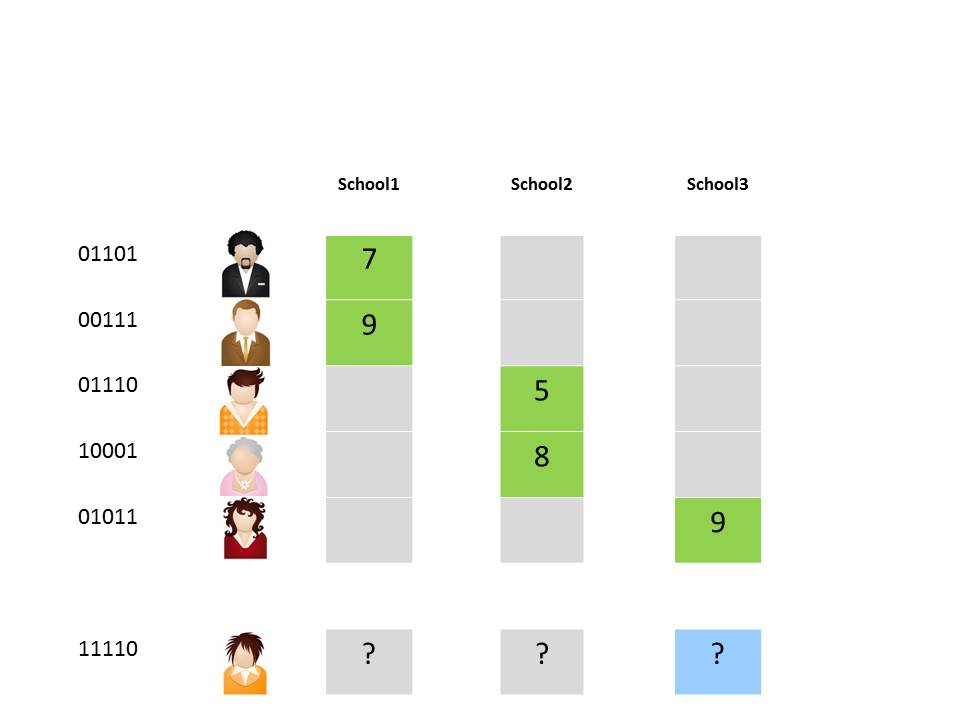
\includegraphics[width=0.9\textwidth,trim = 0 0 100 100,clip]{Figures/pictures/Slide3}
\end{frame}

%\begin{frame}{Conventional MTP settings}
%\begin{definition}[Label ranking] 
%A multi-label classification problem is a specific instantiation of the general framework, which exhibits the following additional properties: 
%\begin{enumerate}
%\item[P5.] The cardinality of $\mathcal{T}$ is $m$; this implies that all targets are observed during training. 
%\item[P6.] No side information is available for targets. Again, without loss of generality, we can hence identify targets with natural numbers, such that the target space is $\mathcal{T} = \{1,...,m\}$. 
%\item[P7.] The score matrix $Y$ has no missing values. 
%\item[P8c.] The score set is $\mathcal{Y} = \{1, \ldots , m\}$, and the scores (interpreted as ranks) are such that $y_{ij} \neq y_{ik}$ for all $1 \leq j,k \neq m$. 
%\end{enumerate}
%\end{definition}
%\end{frame}
%
%
%
%
%
%\begin{frame}{Conventional MTP settings}
%\begin{itemize}
%\item
%In \emph{label ranking}\footnote{E.H., J.\ F\"urnkranz, W.\ Cheng, K.\ Brinker. Label Ranking by Learning Pairwise Preferences, Artificial Intelligence, 172, 2008.}, each instance is associated with a ranking (total order) of the targets.
%\end{itemize}
%%\vspace{0.8cm}
%\begin{center}
%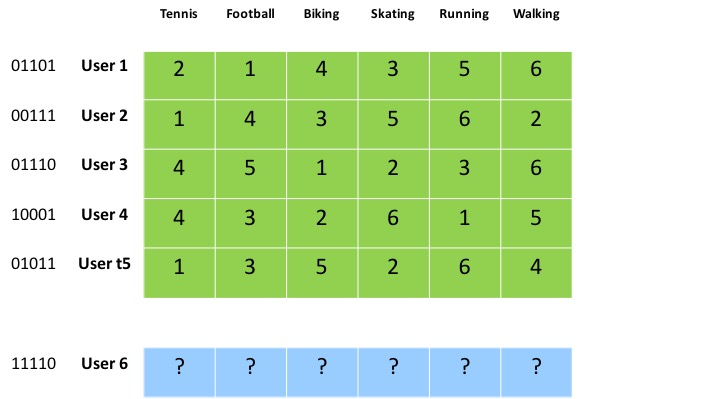
\includegraphics[width=0.8\textwidth]{Figures/pictures/labelranking}
%\end{center}
%\end{frame}





\begin{frame}{Let's assume a document hierarchy: \\
How would you call this machine learning problem?}
\begin{center}
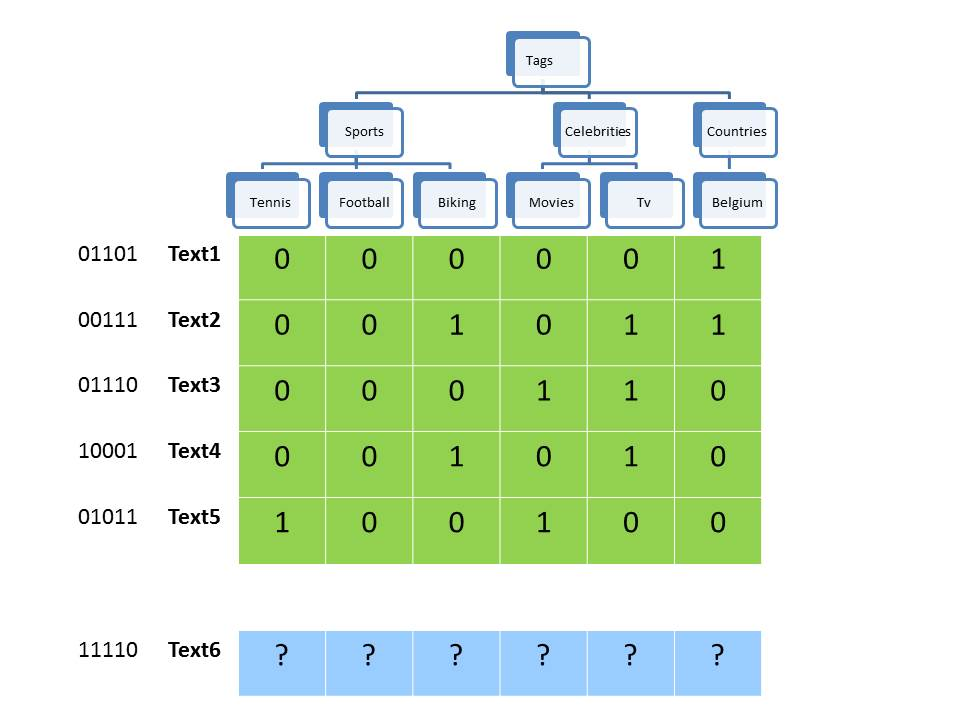
\includegraphics[width=0.75\textwidth,trim = 0 0 100 0,clip]{Figures/pictures/Slide5}
\end{center}
\end{frame}

\begin{frame}{Let's assume a target representation: \\
How would you call this machine learning problem?}
\vspace{0.8cm}
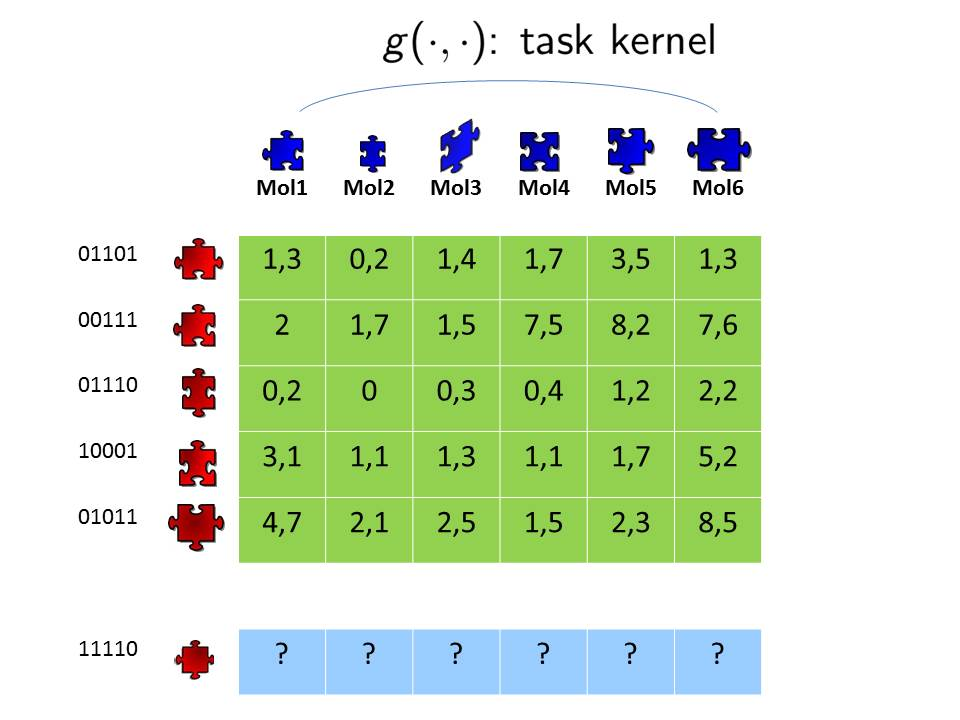
\includegraphics[width=0.9\textwidth,trim = 0 0 0 90,clip]{Figures/pictures/Slide4}

\end{frame}

\begin{frame}{Let's assume a target representation: \\
How would you call this machine learning problem?}
\begin{center}
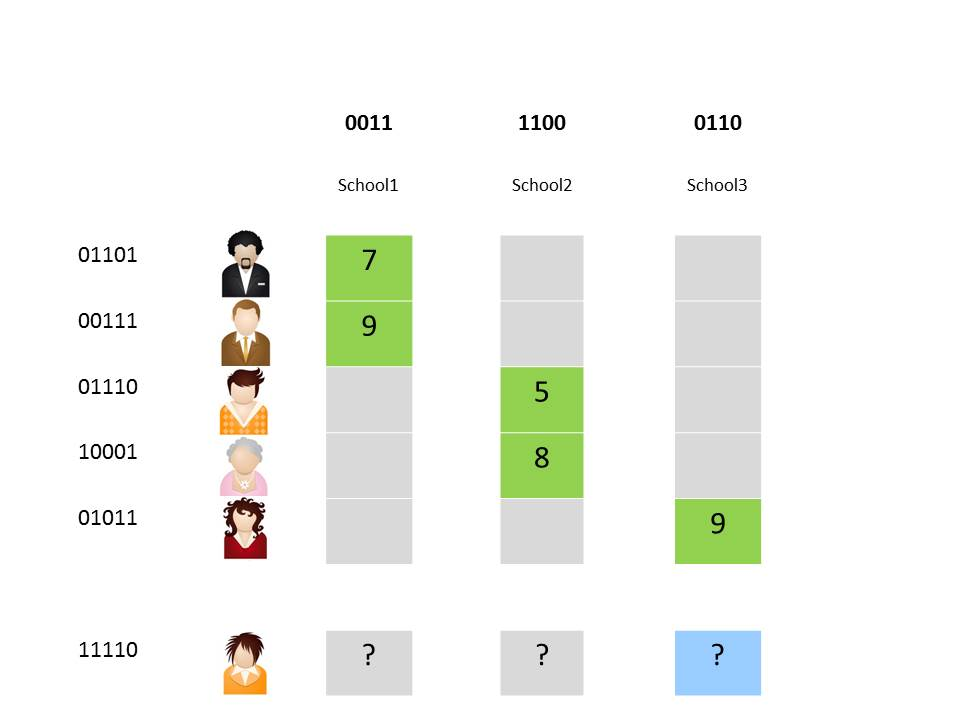
\includegraphics[width=0.8\textwidth,trim = 0 0 100 30,clip]{Figures/pictures/Slide6}
\end{center}

\end{frame}







\begin{frame}{Learning with side information on targets}
\begin{itemize}
\item Additional side information about the target space is available.
\item Examples: 
\begin{itemize}
\item Taxonomy on document categories (\emph{hierarchy}).
\item Representation for the target molecules in drug design application (\emph{structured representation}).
\item Information about schools and courses (geographical location, qualifications of the teachers, reputation of the school, etc.) in student mark forecasting application (\emph{feature representation}).
\end{itemize}
\item Such problems are often referred to as dyadic prediction, link prediction, or network inference settings.
\end{itemize}
\end{frame}
%
%
%\begin{frame}{Learning with side information on targets}
%\begin{itemize}
%\item
%Generally speaking, such settings cover problems that obey the four properties listed in the MTP definition. 
%\item Labels $y_{ij}$ can be arranged in a matrix $Y$, which is often sparse. 
%\item Thus, one may argue that \emph{dyadic prediction} is nothing else than \emph{multi-task learning with task features}. 
%\item However, MTP terminology is rarely used in the dyadic prediction literature. 
%\end{itemize}
%\end{frame}
%
%
%
%
%
%\begin{frame}{Inductive versus transductive learning problems}
%\begin{itemize} 
%\item In the previous problems, 
%\begin{itemize}
%\item predictions need be be generated for novel instances, 
%\item whereas the set of targets is known beforehand and observed during the training phase.
%\end{itemize}
%\item These problems are \emph{inductive} w.r.t.\ instances and \emph{transductive} w.r.t.\ targets.
%\item   
%\emph{Side information} is of crucial importance for generalizing to novel targets that are unobserved during the training phase.
%%such as a novel target molecule in the drug design example, a novel tag in the document annotation example, or a novel course in the student grading example. 
%\end{itemize}
%\end{frame}
%

\begin{frame}{Inductive versus transductive learning problems}
% voorbeeldje met boeken
%\vspace{0.6cm}
$$\qquad g(.,.): \mbox{target similarity}$$

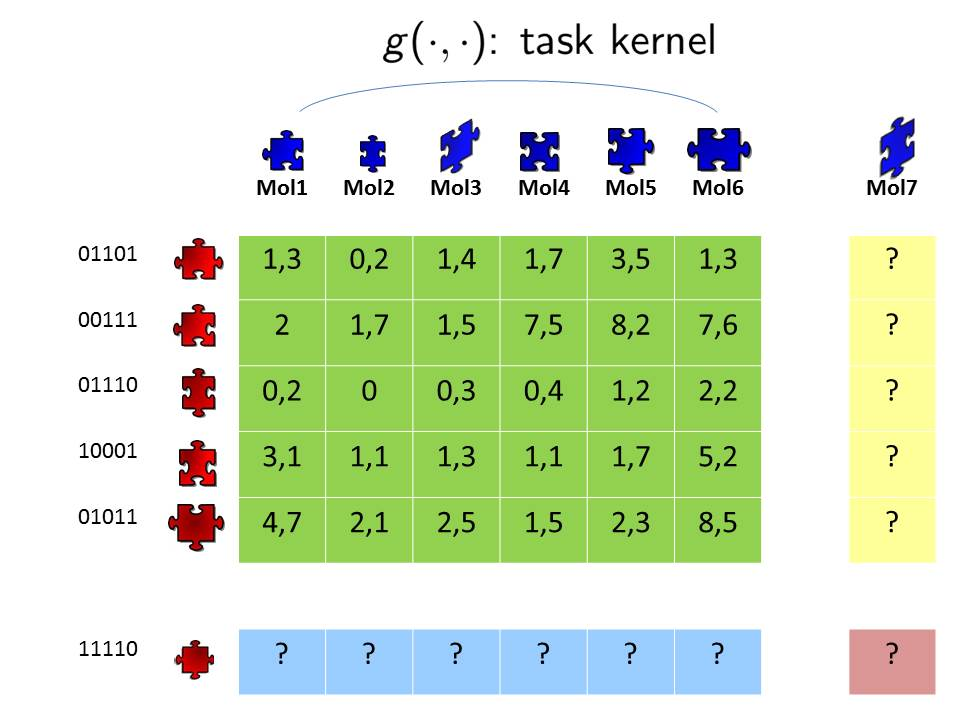
\includegraphics[width=0.9\textwidth,trim = 0 0 0 60,clip]{Figures/pictures/Slide7}
\end{frame}

\begin{frame}{Important subdivision of different learning settings}
   \center
	\vspace{0.4cm}
   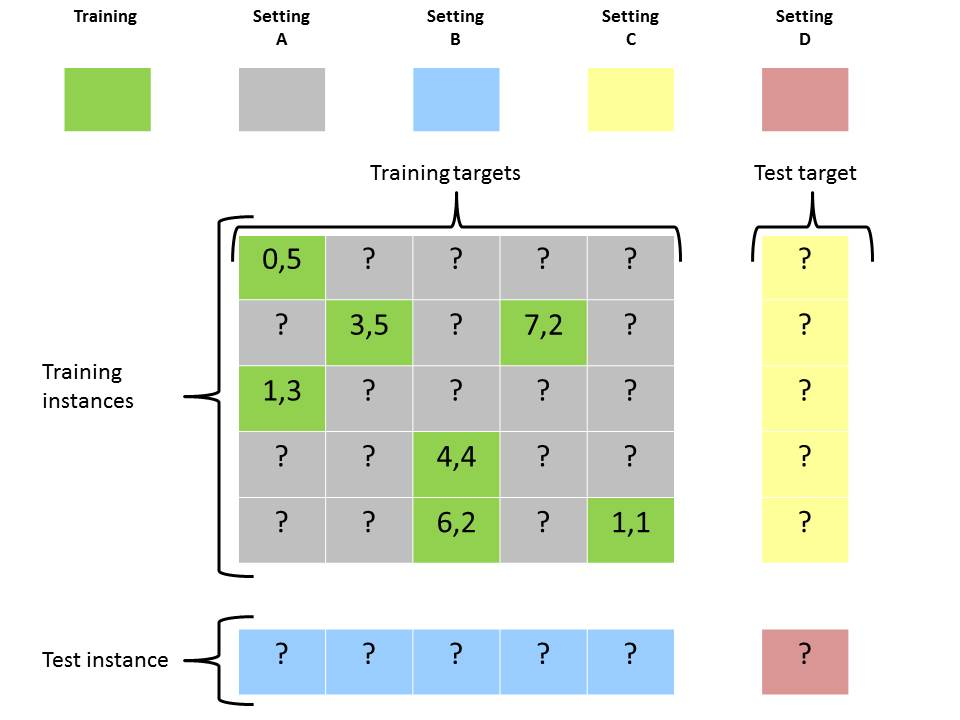
\includegraphics[width=0.9\textwidth]{Figures/pictures/Slide16} % requires the graphicx package
\end{frame}

%
%\begin{frame}{General framework}
%\begin{definition}[Multi-target prediction]
%A multi-target prediction setting is characterized by instances $\vec{x} \in \mathcal{X}$ and targets $\vec{t} \in \mathcal{T}$ with the following properties: 
%\begin{itemize} 
%\item[P1.] A training dataset $\mathcal{D}$ consists of triplets $(\vec{x}_i,\vec{t}_j,y_{ij})$, where $y_{ij} \in \mathcal{Y}$ denotes a score that characterizes the relationship between the instance $\vec{x}_i$ and the target $\vec{t}_j$.  
%\item[P2.] In total, $n$ different instances and $m$ different targets are observed during training, with $n$ and $m$ finite numbers. Thus, the scores $y_{ij}$ of the training data can be arranged in an $n \times m$ matrix $Y$, which is in general incomplete, i.e., $Y$ has missing values.
%\item[P3.] The score set $\mathcal{Y}$ is one-dimensional. It consists of nominal, ordinal or real values.  
%\item[P4.] The goal consists of predicting scores for any instance-target couple $(\vec{x},\vec{t}) \in \mathcal{X} \times \mathcal{T}$.   
%\end{itemize}
%\end{definition}
%
%\end{frame}
%
%
%
%
%\begin{frame}{Specific MTP settings: one example}
%\begin{definition}[Multivariate regression] 
%A multivariate regression problem is a specific instantiation of the general framework, which exhibits the following additional properties: 
%\begin{enumerate}
%\item[P5.] The cardinality of $\mathcal{T}$ is $m$. This implies that all targets are observed during training. 
%\item[P6.] No side information is available for targets. Without loss of generality, we can hence assign the numbers $1$ to $m$ as identifiers to targets, such that the target space is $\mathcal{T} = \{1,...,m\}$. 
%\item[P7.] The score matrix $Y$ has no missing values. 
%\item[P8.] The score set is $\mathcal{Y} = \mathbb{R}$. 
%\end{enumerate}
%\end{definition}
%\end{frame}





\begin{frame}{Inductive versus transductive learning problems}
\begin{definition}[Zero-shot learning]
A zero-shot learning problem is a specific instantiation of the general framework with the following additional property: 
\begin{enumerate}
\item[P5*.] $m < m^* = |\mathcal{T}|$. Some targets are hence not observed during training, but may nevertheless appear at prediction time.  
\end{enumerate}
\end{definition}
\pause

\begin{itemize}
\item By substituting P5 with P5*, one now tackles problems that are inductive instead of transductive w.r.t.\ targets. 
\item The same subdivision can be made for instances. 
\item In total, the four different settings referred to as A, B, C, D can be distinguished (in the presence of side information). %about instances and targets.
\item Theoretically, settings B and C are identical/symmetric, though there are practical differences/asymmetries. 
\end{itemize}
\end{frame}




\begin{frame}{Inductive versus transductive learning problems}
\begin{definition}[Matrix completion]
A matrix completion problem is a specific instantiation of the general framework with the following additional properties: 
\begin{enumerate}
\item[P5.] The cardinality of $\mathcal{T}$ is $m$. This implies that all targets are observed during training. 
\item[P6.] No side information is available for targets. Without loss of generality, we can hence assign identifiers to targets from the set $\{1,...,m\}$ such that the target space is $\mathcal{T} = \{1,...,m\}$.
\item[P9.] The cardinality of $\mathcal{X}$ is $n$. This implies that all instances are observed during training. 
\item[P10.] No side information is available for instances. Without loss of generality, we can hence assign identifiers to instances from the set $\{1,...,n\}$, such that the instance space is $\mathcal{X} = \{1,...,n\}$.
\end{enumerate}
\end{definition}
\end{frame}




\section{A unifying view on MTP methods}


\begin{frame}{Overview of this talk}

\tableofcontents

\end{frame}

\begin{frame}{A unifying view on MTP methods}

\begin{center}

\includegraphics[scale=0.3]{pics/tools}

\begin{tabular}{ll}
\hline
Group of methods & Applicable setting \\
\hline
\hline
\alert{Independent models} & B \\
Similarity-enforcing methods & B   \\ 
Relation-exploiting methods & B and D  \\
Relation-constructing methods & B \\
Representation-exploiting methods & B and D \\
Representation-constructing methods & A and B \\
\hline  
\end{tabular}
\end{center}
\end{frame}

%\begin{frame}{Different learning settings revisited}
   %\center
	%\vspace{0.4cm}
   %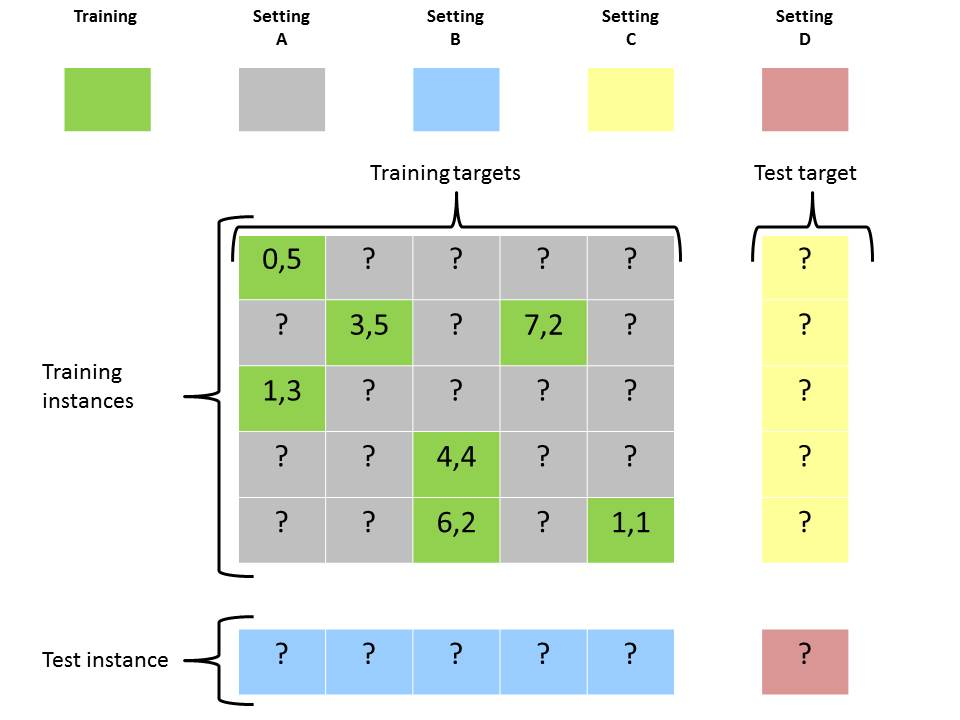
\includegraphics[width=0.9\textwidth]{Figures/pictures/Slide16} % requires the graphicx package
%\end{frame}


\begin{frame}{A baseline method:\\
learning a model for each target independently}
% voorbeeldje met boeken
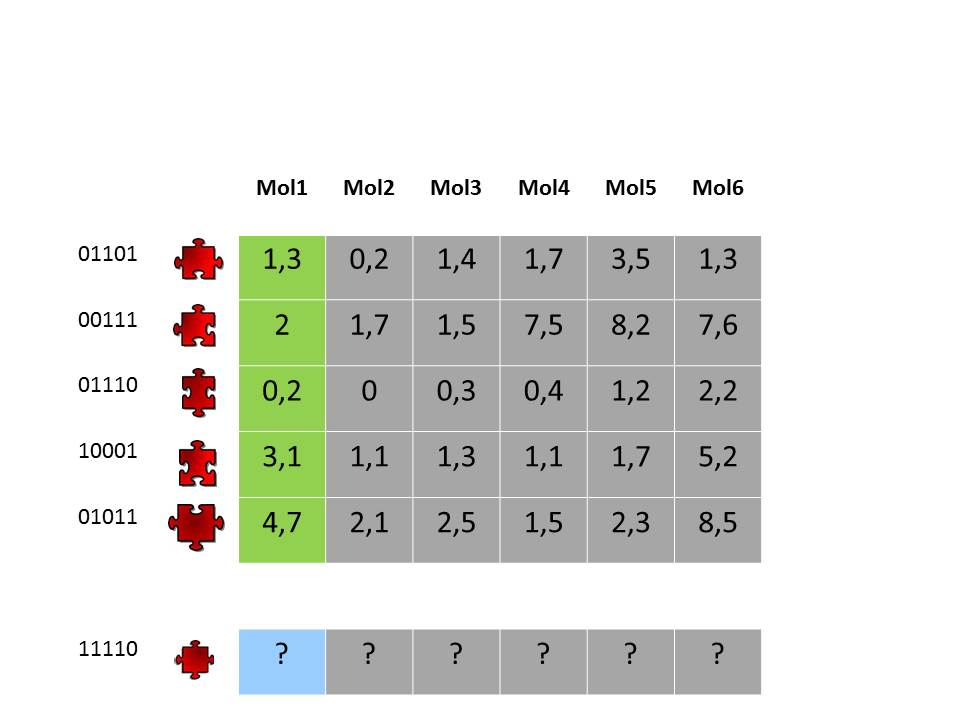
\includegraphics[width=0.9\textwidth,trim = 0 0 100 100,clip]{Figures/pictures/Slide13}
\end{frame}

\begin{frame}{A baseline method:\\
learning a model for each target independently}
% voorbeeldje met boeken
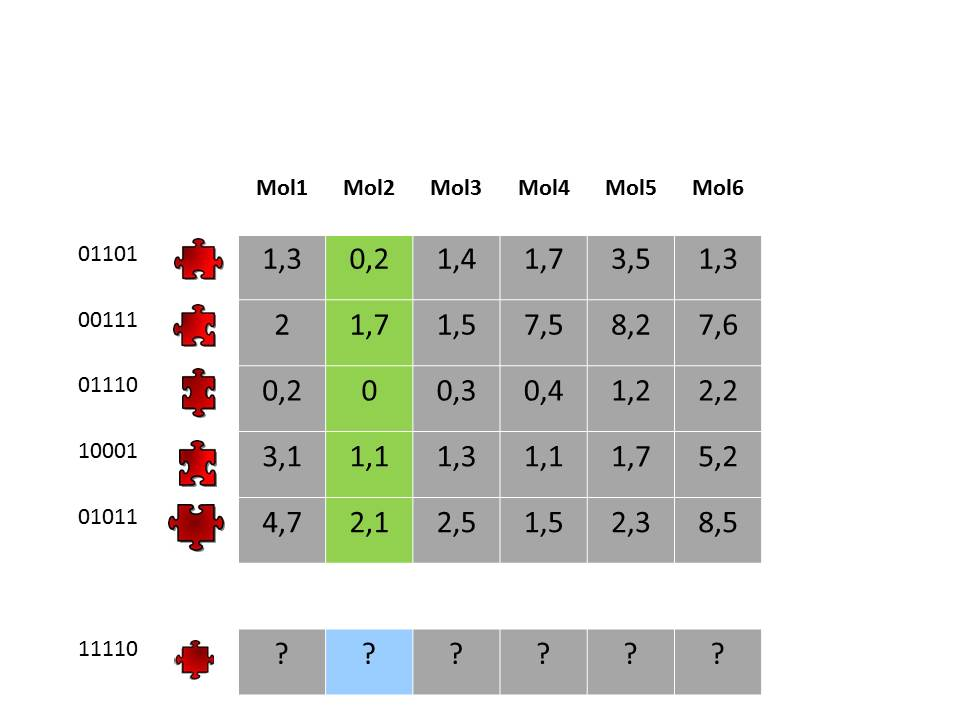
\includegraphics[width=0.9\textwidth,trim = 0 0 100 100,clip]{Figures/pictures/Slide14}
\end{frame}

\begin{frame}{A baseline: Independent Models}
% voorbeeldje met boeken
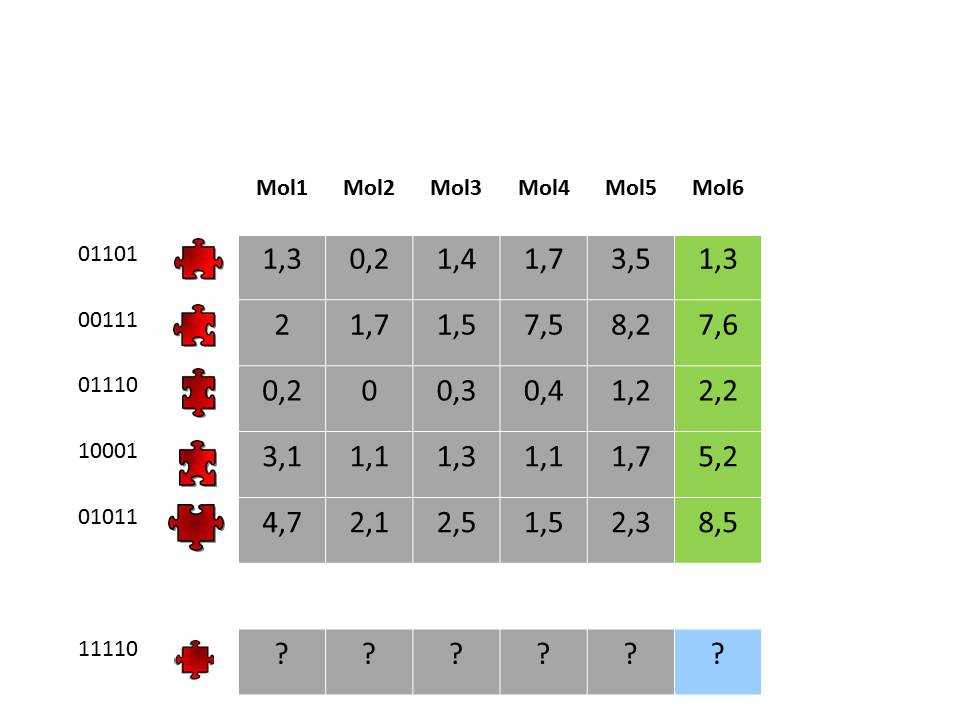
\includegraphics[width=0.9\textwidth,trim = 0 0 100 100,clip]{Figures/pictures/Slide15}
\end{frame}

\begin{frame}{A baseline: Independent Models}
% voorbeeldje met boeken
\vspace{0.5cm}
Linear basis function model for $i$-th target: 
\begin{equation*}
f_i(\vec{x}) = \vec{a}_i^\intercal \phi(\vec{x}) \,,
\label{eq:binrel}
\end{equation*}
Solving as a joint optimization problem: 
\begin{equation*}
\label{eq:multiridge}
\min_A ||Y - XA ||^2_F +  \sum_{i=1}^m \lambda_i \,||\vec{a}_i||^2 \,,
\end{equation*}
$$Y: (n \times m) \qquad  X: (n \times p) \qquad A: (p \times m)$$
With the following notations: 
\begin{equation*}
\label{eq:notation}
X = \begin{bmatrix} \phi(\vec{x}_1)^T \\ \vdots \\ \phi(\vec{x}_n)^T \end{bmatrix} \qquad A = [\vec{a}_1 \quad \cdots \quad \vec{a}_m] \,.
\end{equation*}
%Hamming loss as alternative for binary labels: 
%$${\displaystyle L_{\textit{Ham}}(\vec{y},\hat{\vec{y}}) = \sum_{j=1}^m I(y_j = \hat{y}_j)}$$


\end{frame}

\begin{frame}{The results section of a typical MTP paper...}
\begin{center}
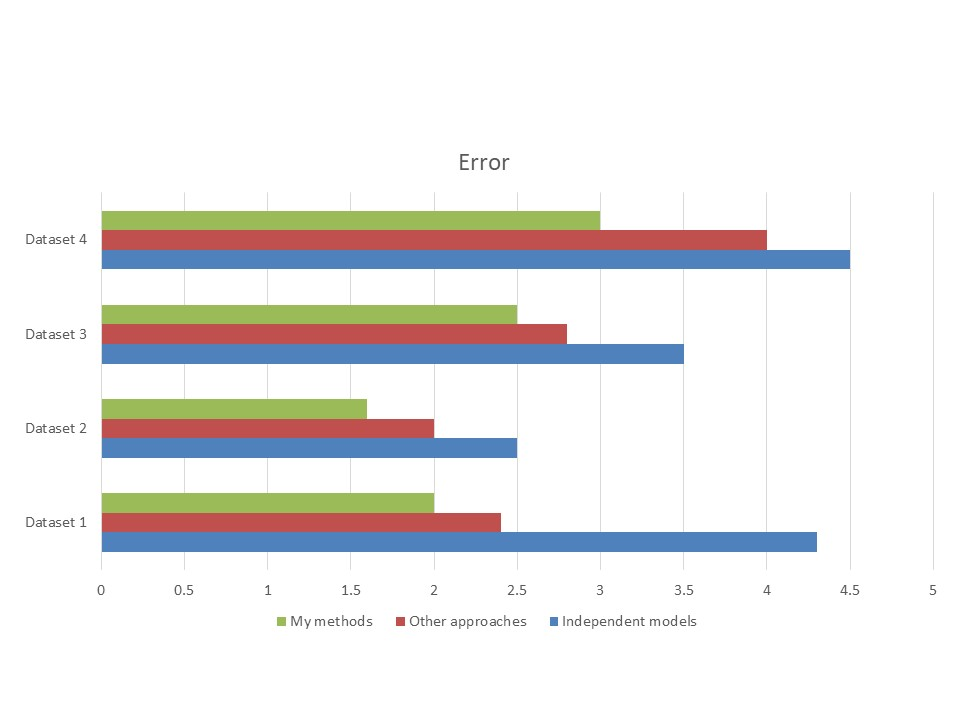
\includegraphics[scale=0.45, trim = 0 50 0 100,clip]{Figures/barplots} \\

Independent models a.k.a.\ binary relevance, models that do not exploit target dependencies, one-versus-all, etc.
\end{center}
\end{frame}


\begin{frame}

\begin{center}
Learning a model for each target independently is still state-of-the-art in extreme multi-label classification\footnote{Babbar and Sch\"olkopf, DISMEC: Distributed Sparse Machines for Extreme Multi-label classification, WSDM 2017}:

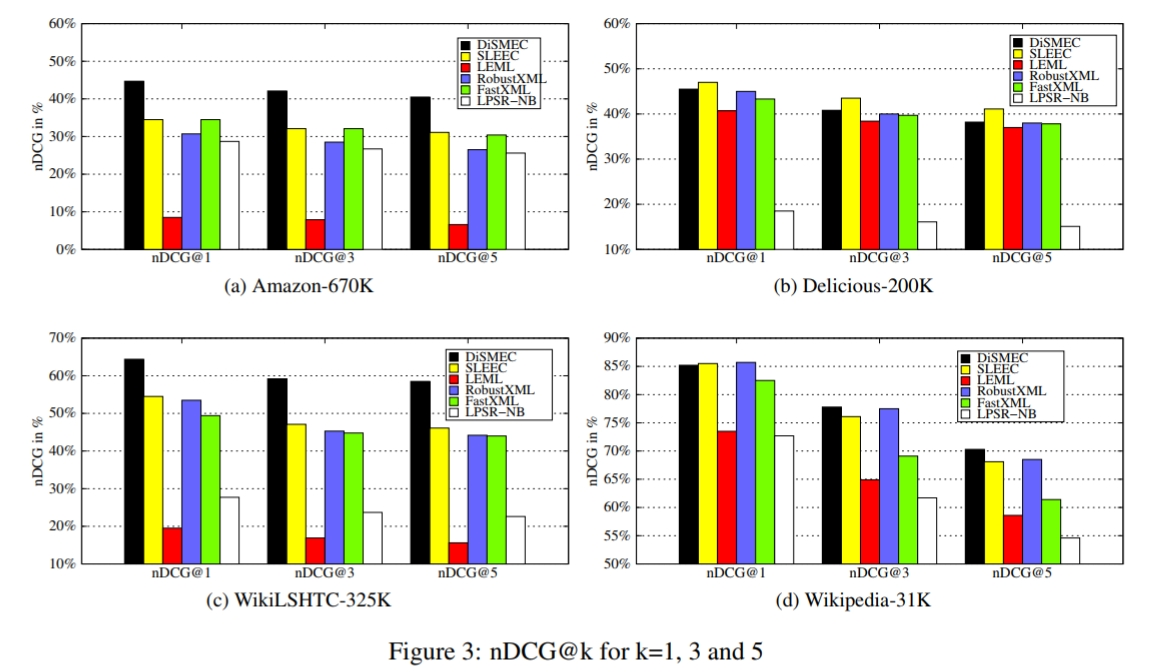
\includegraphics[scale=0.3]{Figures/dismec} 
\end{center}

\end{frame}

%%%%%%%%%%%%%%%%%%%%%%%%%%%%%%%%%%%%%%%%%%%%%%%%%%%%%%%%%%%%%%%%%%%%%%%%%%%%%% 
%%%%%%%%%%%%%%%%%%%%%%%%%%%%%%%%%%%%%%%%%%%%%%%%%%%%%%%%%%%%%%%%%%%%%%%%%%%%%% 

%%%%%%%%%%%%%%%%%%%%%%%%%%%%%%%%%%%%%%%%%%%%%%%%%%%%%%%%%%%%%%%%%%%%%%%%%%%%%% 
%%%%%%%%%%%%%%%%%%%%%%%%%%%%%%%%%%%%%%%%%%%%%%%%%%%%%%%%%%%%%%%%%%%%%%%%%%%%%% 
%\frame{
  %\frametitle{ DiSMEC - Distributed Sparse Machines for XMC }
%
%\begin{algorithmic}[1]
 %\Require  {Training data $\mathcal{T} = \{(\vec{x}_1,\vec{y}_1) \ldots (\vec{x}_n,\vec{y}_n) \}$, input dimensionality $p$, label set $\{1 \ldots m\}$, $B=\lfloor\frac{m}{1000}\rfloor+1$  and pruning threshold $\Delta$}
%
%\Ensure{Learnt $p \times m$ matrix $A$ in sparse format} \pause 
%
%\State Load single copy of input vectors $X = \{\vec{x}_1 \ldots \vec{x}_n \}$ in the main memory  %\Comment{\textit{Refactor data without replication}} 
%
%\State Load binary sign vectors $\vec{s}_{j} = \{+1,-1\}_{i=1}^n$ separately for each label \pause 
%
%\For{$\{b=0; b < B; b++ \}$} \Comment{\alert{1st parallelization}}
%
        %\State \#pragma omp parallel for private($j$)  \Comment{\alert{2nd parallelization}}
%
       %\For{$\{j=b\times1000; j \leq (b + 1)\times1000; j++ \}$}
%
%\State Using $(\vec{X}, \vec{s}_{j})$, train weight vector $\vec{a}_{j}$ on a single core
%
%\State \alert{Prune ambiguous weights} in $\vec{a}_{j}$ 
%\EndFor
%
%\State \Return $p \times 1000$ matrix $A$  
%
%\EndFor
%
%\State \Return $p \times m$ weight matrix $A$ 
%\end{algorithmic} \pause 
%\begin{itemize} 
%\item Learns model for LSHTCWiki-325K in 6 hours on 400 cores
%\item Model size is 3GB due to pruning step
%\end{itemize}
%}
%
%\frame{
  %\frametitle{ Distribution of Learnt Weights}
%
%\begin{columns}
%\column{0.5\columnwidth}
%\begin{figure}[ht]
%\centering
%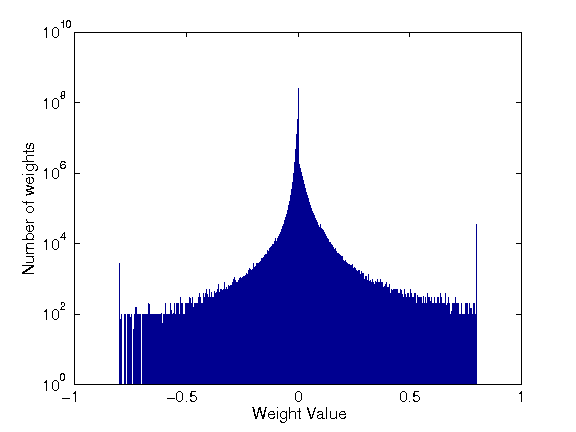
\includegraphics[width=\textwidth]{Figures/wiki10nonsparabs0p8.png}
%\caption{Before pruning}
%\end{figure}
%
%%\end{itemize}
%\column{0.5\columnwidth}
%\begin{figure}[ht]
%\centering
%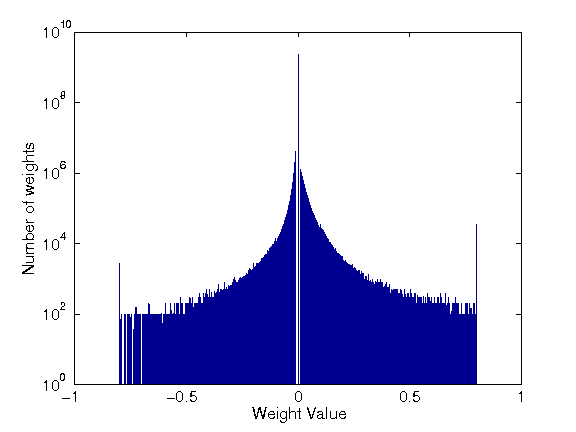
\includegraphics[width=\textwidth]{Figures/l2c1abs0p8.png}
%\caption{After pruning small weights}
%\end{figure}
%\end{columns}
%\begin{itemize}
%\item Of the 3 Billion weights, 97\% are s.t, $A_ij \leq |0.01|$, and hence non-discriminative
%\item Storing them leads to large model sizes but no benefit in classification
%\end{itemize}
%
%}




\begin{frame}{A unifying view on MTP methods}

\begin{center}

\includegraphics[scale=0.3]{pics/tools}

\begin{tabular}{ll}
\hline
Group of methods & Applicable setting \\
\hline
\hline
Independent models & B \\
\alert{Similarity-enforcing methods} & B   \\ 
Relation-exploiting methods & B and D  \\
Relation-constructing methods & B \\
Representation-exploiting methods & B and D \\
Representation-constructing methods & A and B \\
\hline  
\end{tabular}
\end{center}
\end{frame}



%
%\begin{frame}{Learning a model for each target independently with kernel ridge regression}
%
%
%\begin{itemize}
%\item Model for target $\bm{t}_j$:
%$$ \predfun_j^{\text{IT}}(\bm{d}) = \sum_{i=1}^{\osize}
%a_{ij}^\text{IT} \kernelf(\bm{d},\bm{d}_i) $$
%\item[] $\osize$: number of labeled instances per target
%\item[] $\lsize$: number of targets
 %\item[] $\bm{d}_i$: feature representation of instance $i$ 
%\item[] $\kernelf(\cdot,\cdot)$: a kernel for instances \pause 
%\item[]
%\item Optimization problem:
%$$
 %\min_{\mathbf{A}} \| \mathbf{Y} - \mathbf{KA} \|_F^2 + \regparam_d \trace[{\bm{A}}\transpose\dkernelm\bm{A}] $$
%%with $\bm{A}^\text{IT}=[a_{ij}^\text{IT}]\in\mathbb{R}^{\osize\times\qsize}$ and  for the instances 
%\item[] $\bm{Y}_{.j}\in\mathbb{R}^\osize$: the labels of target $\bm{t}_j$ 
%\item[] $\dkernelm \in\mathbb{R}^{\osize\times\osize}$: the Gram matrix of instance kernel $\kernelf(\cdot,\cdot)$ 
%%\item Solving the following linear system:
%%$$\left(\dkernelm+\regparam_d\idmatrix\right)\bm{A}^\text{IT}=\bm{Y}$$
%\end{itemize}
%\end{frame}


%\begin{frame}
%\frametitle{Multi-target prediction methods }
%
%\begin{itemize}
%\item Methods that exploit the similarities between the structural parts of target models:
%\begin{equation}
%\label{eqn:slp_1}
%\vec{y} = \mathbf{h} (\mathbf{f}(\vec{x}), \vec{x})\,,
%\end{equation}
%where $\mathbf{f}(\vec{x})$ is the prediction vector obtained by univariate methods, and  $\mathbf{h}(\cdot)$ are additional shrunken or regularized classifiers.
%\item Alternatively, a similar model can be given by:
%\begin{equation}
%\label{eqn:slp_2}
%\mathbf{h}^{-1}(\vec{y}, \vec{x}) = \mathbf{f}(\vec{x})\,,
%\end{equation}
%i.e., the output space (possibly along with the feature space) is first transformed, and than univariate (regression) methods are then trained on the new output variables $\mathbf{h}^{-1}(\vec{y}, \vec{x})$. 
%\end{itemize}
%
%\end{frame}






\begin{frame}[fragile]
\frametitle{Mean-regularized multi-task learning\footnote{Evgeniou and Pontil, Regularized multi--task learning, KDD 2004.}}

\vspace{0.2cm}
\begin{columns}
\column{5cm}
\small{
\begin{itemize}
\item \emph{Simple assumption}: models for different targets are related to each other.
\item \emph{Simple solution}: the parameters of these models should have similar values.
\item \emph{Approach}: bias the parameter vectors towards their mean vector.
%\item \emph{Disadvantage}: the assumption of all target models being similar might be invalid for many applications.
\end{itemize}
}
\column{5.5cm}

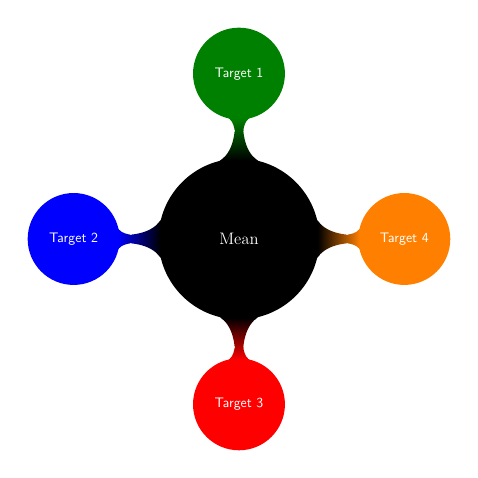
\begin{tikzpicture}[
  level 1 concept/.append style={font=\sf, level distance = 21mm},
  level 2 concept/.append style={font=\sf, level distance = 21mm},
  every node/.append style={scale=0.5}]

  \path[mindmap, concept color=black,text=white]

    node[concept] {Mean}
    child[grow = 90, concept color=green!50!black] { node[concept] {Target 1}}
    child[grow = 180,concept color=blue] { node[concept] {Target 2}}
	child[grow = 270,concept color=red] { node[concept] {Target 3} }
	child[grow = 360,concept color=orange] { node[concept] {Target 4} };   
\end{tikzpicture}
\end{columns}
\vspace{0.2cm}
\begin{equation*}
\label{eq:meanreg}
\min_A ||Y - XA ||^2_F + \lambda \sum_{i=1}^m ||\vec{a}_i - \frac{1}{m} \sum_{j=1}^m \vec{a}_j||^2 \, ,
\end{equation*}
\end{frame}

\begin{frame}{Joint feature selection}
\begin{itemize}
\item Enforce that the same features are selected for different targets\footnote{Obozinski et al. Joint covariate selection and joint subspace selection
for multiple classification problems. Statistics and Computing 2010}:
$$
\min_A ||Y - XA ||^2_F + \lambda \sum_{j=1}^p ||\vec{a}_j||^2  
$$ \pause 
\item The vectors $\vec{a}_j$ now represent the columns of matrix $A^T$:
\end{itemize}
\begin{center}
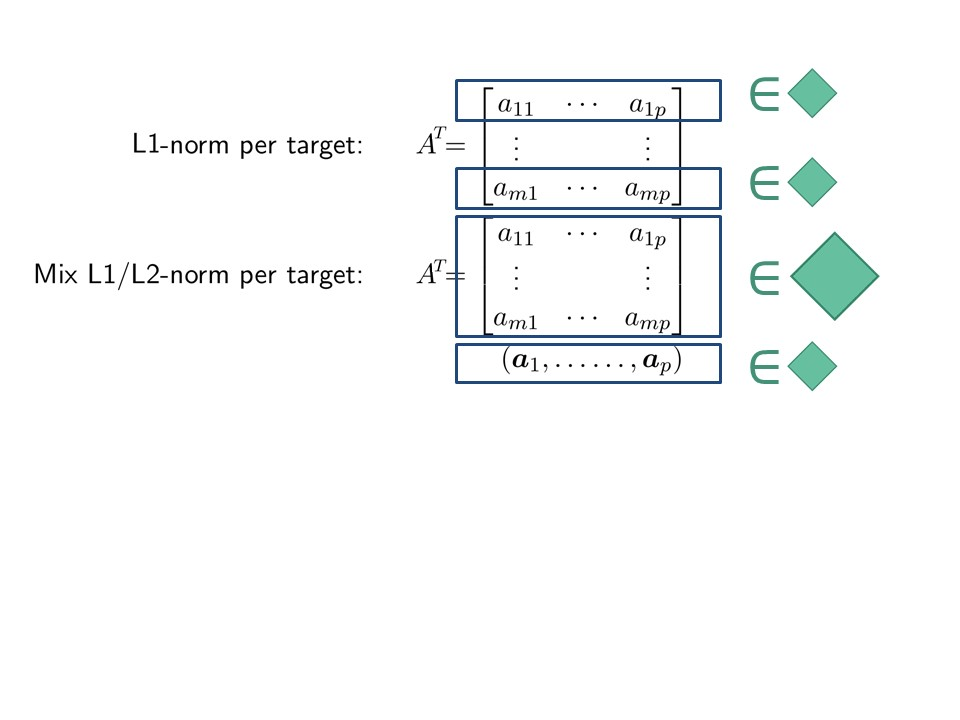
\includegraphics[width=0.9\textwidth,trim = 0 240 30 50,clip]{Figures/pictures/Dia21}
\end{center}
%\begin{eqnarray*}
%\mbox{L2-norm per target:} && 
%A= \begin{bmatrix}
%a_{11} & \cdots & a_{1p} \\
%\vdots & & \vdots \\
%a_{m1} & \cdots & a_{mp}
%\end{bmatrix} \\
%\mbox{Mix L1/L2-norm per target:} && 
%A= \begin{bmatrix}
%a_{11} & \cdots & a_{1p} \\
%\vdots & & \vdots \\
%a_{m1} & \cdots & a_{mp}
%\end{bmatrix}\\
%&& \quad \qquad  (\vec{a}_1,\ldots \ldots,\vec{a}_p)
%\end{eqnarray*}
%$$
\end{frame}


\begin{frame}
\frametitle{Stacking (Stacked generalization)}

\begin{itemize}
\item Originally introduced as a general ensemble learning or blending technique.\footnote{Wolpert, Stacked generalization. Neural Networks 1992}
\item Level 1 classifiers: apply a series of ML methods on the same dataset (or, one ML method on bootstrap samples of the dataset)
\item Level 2 classifier: apply an ML method to a new dataset consisting of the predictions obtaining at Level 1 
\end{itemize}

\begin{center}
\def\layersep{1.25cm}
\begin{tikzpicture}[shorten >=1pt,->,draw=black!50, node distance=\layersep]
    \tikzstyle{every pin edge}=[<-,shorten <=1pt]
    \tikzstyle{neuron}=[circle,fill=black!25,minimum size=17pt,inner sep=0pt]
    \tikzstyle{input neuron}=[neuron, fill=green!50];
    \tikzstyle{output neuron}=[neuron, fill=red!50];
    \tikzstyle{hidden neuron}=[neuron, fill=blue!50];
    \tikzstyle{annot} = [text width=4em, text centered]

   % Draw the input layer nodes
   \foreach \name / \y in {1,...,4}
    % This is the same as writing \foreach \name / \y in {1/1,2/2,3/3,4/4}
        \node[input neuron] (I-\name) at (\y, 0) {$f_\y$};

    % Draw the hidden layer nodes
   \foreach \name / \y in {1}
      % \path%[yshift=0.5cm]
           \node[hidden neuron] (H-\name) at (2.5, \layersep) {$h_\y$};


% % Draw the output layer node
    \node[output neuron] (I) at (2.5, -\layersep) {$\bx$};
%%
%%    % Connect every node in the input layer with every node in the
%%    % hidden layer.
     \foreach \source in {1,...,4}
        \foreach \dest in {1}
            \path (I-\source) edge (H-\dest);
%%
%    % Connect every node in the hidden layer with the output layer
  \foreach \source in {1,...,4}
     \path (I) edge (I-\source);
%
   % Annotate the layers
  \node[annot,left of=H-1, node distance=3cm] (hl) {Level 2}; 
   \node[annot,below of=hl, node distance=\layersep] {Level 1};
%%    \node[annot,right of=hl] {Output layer};
\end{tikzpicture}
\end{center}

%D. Wolpert, Stacked Generalization, Machine Learning, 1992
\end{frame}

\begin{frame}
\frametitle{Stacking applied to multi-target prediction\footnote{Cheng and H\"ullermeier, Combining Instance-based learning and Logistic Regreession for Multi-Label classification, Machine Learning, 2009} }

\begin{columns}
\begin{column}{5cm}
\begin{itemize}
\item Level 1 classifiers: learn a model for every target independently 
\item Level 2 classifier: learn again a model for every target independently, using the predictions of the first step as features
\end{itemize}
\end{column}

\begin{column}{6cm}
\def\layersep{2.5cm}
\begin{tikzpicture}[shorten >=1pt,->,draw=black!50, node distance=\layersep]
    \tikzstyle{every pin edge}=[<-,shorten <=1pt]
    \tikzstyle{neuron}=[circle,fill=black!25,minimum size=17pt,inner sep=0pt]
    \tikzstyle{input neuron}=[neuron, fill=green!50];
    \tikzstyle{output neuron}=[neuron, fill=red!50];
    \tikzstyle{hidden neuron}=[neuron, fill=blue!50];
    \tikzstyle{annot} = [text width=4em, text centered]

   % Draw the input layer nodes
   \foreach \name / \y in {1,...,4}
    % This is the same as writing \foreach \name / \y in {1/1,2/2,3/3,4/4}
        \node[input neuron] (I-\name) at (\y, 0) {$f_\y$};

    % Draw the hidden layer nodes
   \foreach \name / \y in {1,...,4}
      % \path%[yshift=0.5cm]
           \node[hidden neuron] (H-\name) at (\y, \layersep) {$h_\y$};


% % Draw the output layer node
    \node[output neuron] (I) at (2.5, -\layersep) {$\bx$};
%%
%%    % Connect every node in the input layer with every node in the
%%    % hidden layer.
     \foreach \source in {1,...,4}
        \foreach \dest in {1,...,4}
            \path (I-\source) edge (H-\dest);
%%
%    % Connect every node in the hidden layer with the output layer
  \foreach \source in {1,...,4}
     \path (I) edge (I-\source);
%
   % Annotate the layers
  \node[annot,left of=H-1, node distance=1cm] (hl) {Level 2}; 
   \node[annot,left of=I-1, node distance=1cm] {Level 1};
%%    \node[annot,right of=hl] {Output layer};
\end{tikzpicture}
\end{column}
\end{columns}

% 


\end{frame}

%
%\begin{frame}
%\frametitle{Stacking applied to multi-target prediction: general principle\footnote{Cheng and Huellermeier, Combining Instance-based learning and Logistic Regreession for Multi-Label classification, Machine Learning, 2009}}
%
%\begin{center}
%\def\layersep{2.5cm}
%\begin{tikzpicture}[shorten >=1pt,->,draw=black!50, node distance=\layersep]
    %\tikzstyle{every pin edge}=[<-,shorten <=1pt]
    %\tikzstyle{neuron}=[circle,fill=black!25,minimum size=17pt,inner sep=0pt]
    %\tikzstyle{input neuron}=[neuron, fill=green!50];
    %\tikzstyle{output neuron}=[neuron, fill=red!50];
    %\tikzstyle{hidden neuron}=[neuron, fill=blue!50];
    %\tikzstyle{annot} = [text width=4em, text centered]
%
   %% Draw the input layer nodes
   %\foreach \name / \y in {1,...,4}
    %% This is the same as writing \foreach \name / \y in {1/1,2/2,3/3,4/4}
        %\node[input neuron] (I-\name) at (\y, 0) {$f_\y$};
%
    %% Draw the hidden layer nodes
   %\foreach \name / \y in {1,...,4}
      %% \path%[yshift=0.5cm]
           %\node[hidden neuron] (H-\name) at (\y, \layersep) {$h_\y$};
%
%
%% % Draw the output layer node
    %\node[output neuron] (I) at (2.5, -\layersep) {$\bx$};
%%%
%%%    % Connect every node in the input layer with every node in the
%%%    % hidden layer.
     %\foreach \source in {1,...,4}
        %\foreach \dest in {1,...,4}
            %\path (I-\source) edge (H-\dest);
%%%
%%    % Connect every node in the hidden layer with the output layer
  %\foreach \source in {1,...,4}
     %\path (I) edge (I-\source);
%%
   %% Annotate the layers
  %\node[annot,left of=H-1, node distance=1cm] (hl) {Level 2}; 
   %\node[annot,left of=I-1, node distance=1cm] {Level 1};
%%%    \node[annot,right of=hl] {Output layer};
%\end{tikzpicture}
%\end{center}
%
%% 
%
%
%\end{frame}

\begin{frame}{Enforcing similarity in (Deep) Neural Networks}
\begin{center}
Commonly-used architecture: weight sharing among targets\footnote{Caruana, Multitask learning: A knowledge-based source of inductive bias. Machine
Learning 1997} \\
\vspace{0.2cm}
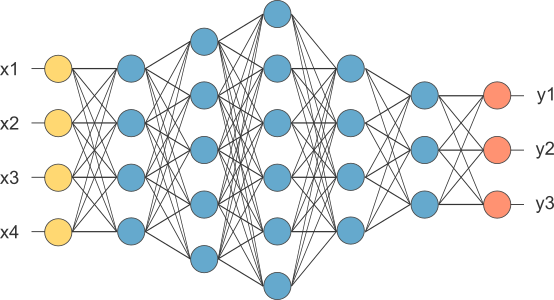
\includegraphics[scale=0.6]{Figures/weightsharing}
\end{center}
\end{frame}

\begin{frame}{Re-using Pretrained Models in (Deep) Neural Networks}
\begin{center}
Commonly-used training method: first train on targets that have a lot of observations, only train some parameters for targets that have few observations \footnote{Keras Tutorial: Transfer Learning using pre-trained models } \\
%\vspace{0.2cm}
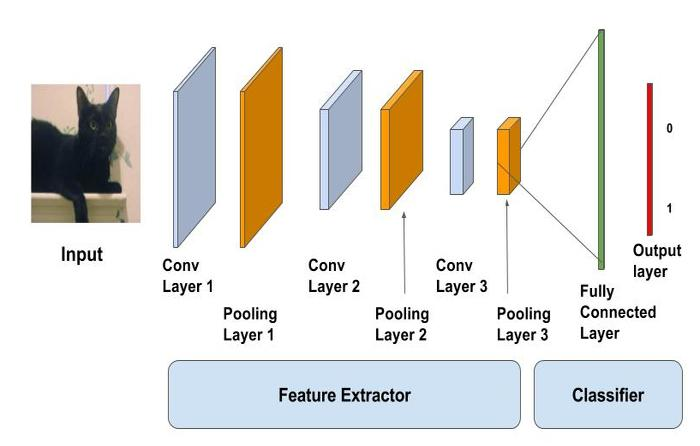
\includegraphics[scale=0.4]{Figures/pretrain2}
\end{center}
\end{frame}

\begin{frame}

\begin{center}

\includegraphics[scale=0.5]{Figures/interaction}
\end{center}
\begin{exampleblock}{Question}
In which situations are similarity-enforcing models capable of outperforming independent models w.r.t.\ predictive performance? 
\begin{itemize}
\item Always
\item When $p$ is sufficiently large
\item When $m$ is sufficiently large
\item When the targets are sufficiently correlated
\end{itemize}
\end{exampleblock}
\end{frame}

\begin{frame}
\frametitle{An intuitive explanation: James-Stein estimation}

\begin{itemize}
\item Consider a sample of a multivariate normal distribution $\by \sim N(\vec{\theta}, \sigma^2\mathbf{I})$.
\begin{center}
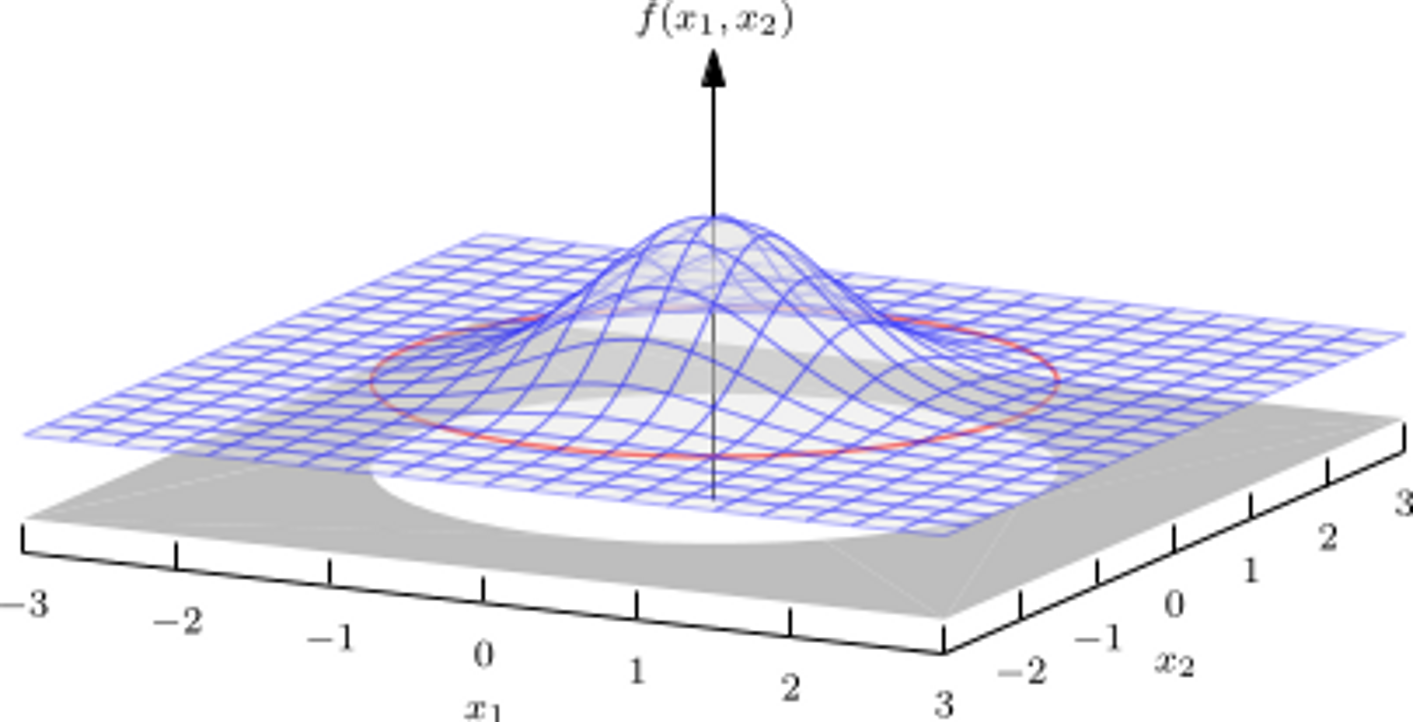
\includegraphics[width = 4.5cm]{Figures/biva}
\end{center}
\item What is the best estimator of the mean vector $\vec{\theta}$?
\item Evaluation w.r.t. MSE: $\mathbb{E}[(\vec\theta - \hat{\vec\theta})^2]$ \pause 
\item Single-observation maximum likelihood estimator: $\hat{\vec\theta}^{\mathrm{ML}} = \by$ \pause 
\item James-Stein estimator\footnote{W. James and C. Stein. Estimation with quadratic loss. In Proc. Fourth Berkeley Symp. Math.
Statist. Prob. 1, pages 361-379, 1961}: 
$$
\hat{\theta}^{\mathrm{JS}} = \left (1 - \frac{(m-2)\sigma^2}{\|\by\|^2} \right )\by
$$
\end{itemize}

\end{frame}




\begin{frame}


\begin{itemize}
%\item Similar principle as many target regularization methods.

\item Works best when the norm of the mean vector is close to zero:\\
\begin{center}
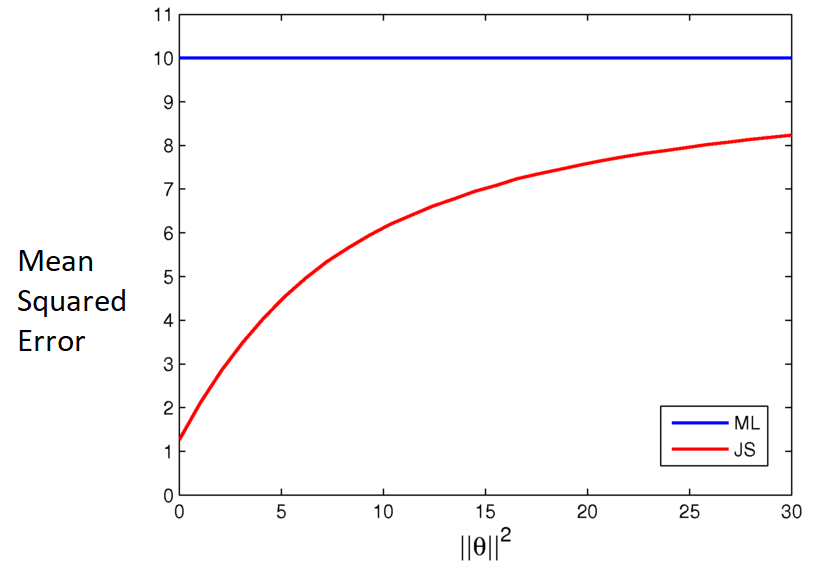
\includegraphics[width=7cm]{Figures/JS}
\end{center} \pause 
\item Regularization towards other directions is also possible:
$$
\hat{\theta}^{\mathrm{JS+}} = \left (1 - \frac{(m-2)\sigma^2}{\|\by - \vec{v}\|^2} \right )(\by - \vec{v}) + \vec{v}
$$
\item Only outperforms the maximum likelihood estimator w.r.t. the sum of squared errors over all components, \alert{and only when $m \geq 3$}
%\item Does not outperform the squared error when evaluating an individual component (i.e. one target).

\end{itemize}
\end{frame}

\begin{frame}{A unifying view on MTP methods}

\begin{center}

\includegraphics[scale=0.3]{pics/tools}

\begin{tabular}{ll}
\hline
Group of methods & Applicable setting \\
\hline
\hline
Independent models & B \\
Similarity-enforcing methods & B   \\ 
\alert{Relation-exploiting methods} & B and D  \\
Relation-constructing methods & B  \\
Representation-exploiting methods & B and D \\
Representation-constructing methods & A and B \\
\hline  
\end{tabular}
\end{center}
\end{frame}

\begin{frame}{Different learning settings revisited}
   \center
	\vspace{0.4cm}
   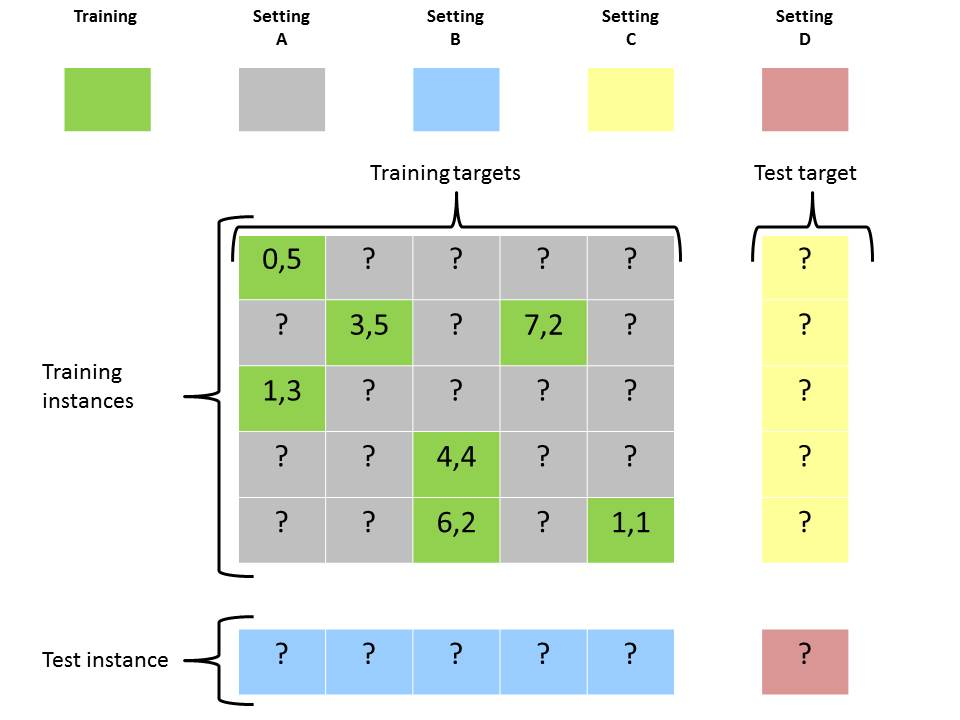
\includegraphics[width=0.9\textwidth]{Figures/pictures/Slide16} % requires the graphicx package
\end{frame}


\begin{frame}{An example from the introduction revisited}
\begin{center}
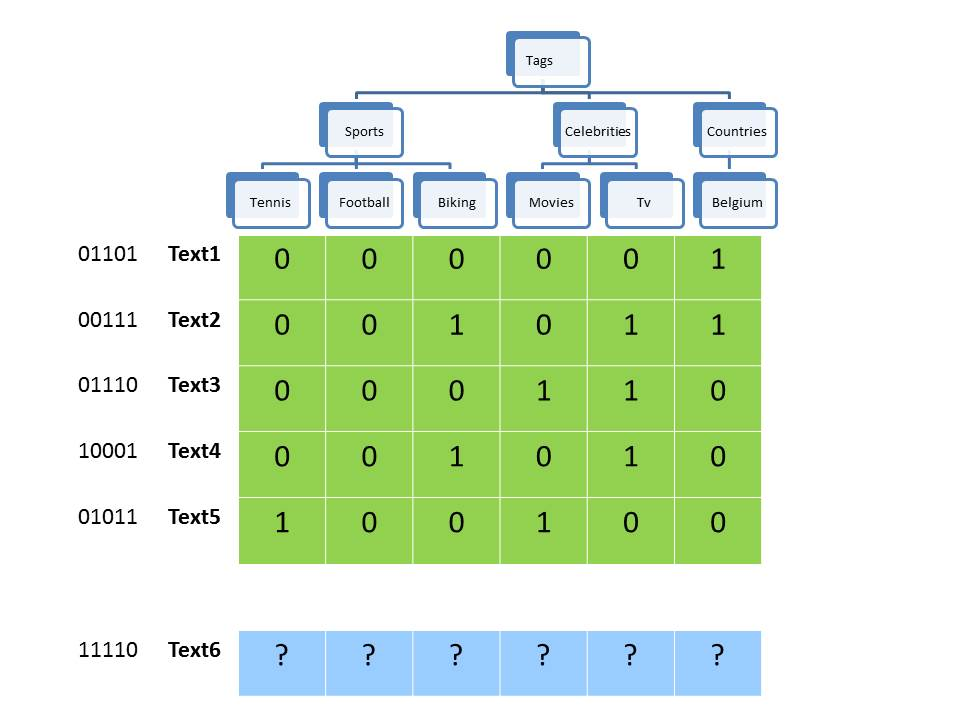
\includegraphics[width=0.75\textwidth,trim = 0 0 100 0,clip]{Figures/pictures/Slide5}
\end{center}
\end{frame}

\begin{frame}{Exploiting relations in regularization terms}

\begin{center}
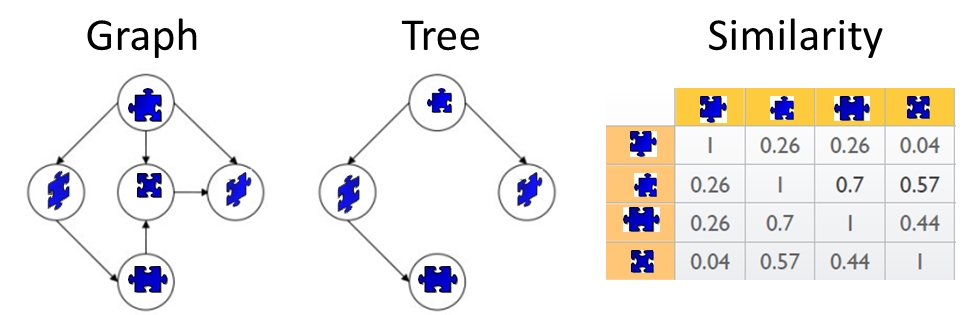
\includegraphics[width=\textwidth]{pics/targetrelations}
\end{center} \pause 

Graph-based regularization is an approach that can be applied to the three types of relations\footnote{Gopal and Yang, Recursive regularization for large-scale classification with hierarchical
and graphical dependencies, KDD 2013}: 
\begin{equation*}
\min_A ||Y - XA ||^2_F + \lambda \sum_{i=1}^m \sum_{j \in \mathcal{N}(i)} ||\vec{a}_i - \ \vec{a}_j||^2 
\end{equation*}

\end{frame}

\begin{frame}{Hierarchical multi-label classfication}

\vspace{-0.2cm}
\begin{center}
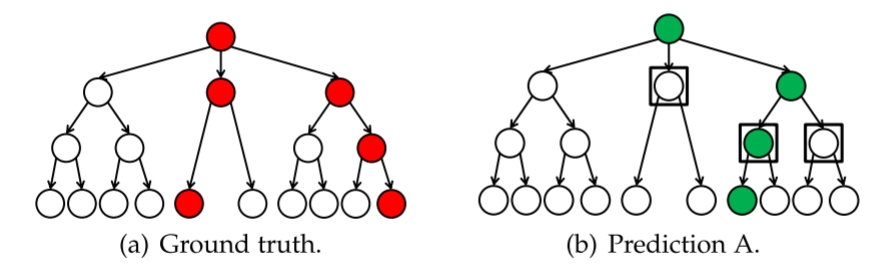
\includegraphics[width=\textwidth]{Figures/hloss}
\end{center}

\vspace{-0.2cm}
In addition to performance gains in general, hierarchies can also be used to define specific loss functions, such as the H-loss\footnote{Bi and Kwok, Bayes-optimal hierarchical multi-label classification, IEEE Transactions on Knowledge and Data Engineering, 2014}: 
$$\ell_{Hier}(\vec{y},\hat{\vec{y}}) = \sum_{j: y_j \neq \hat{y_j}} c_j \, \assert{\textit{anc}(y_j) = \textit{anc}(\hat{y}_j)}$$
$c_i$ depends on the depth of node $i$
\end{frame}

\begin{frame}{Exploiting similarity measures among targets}

\begin{center}
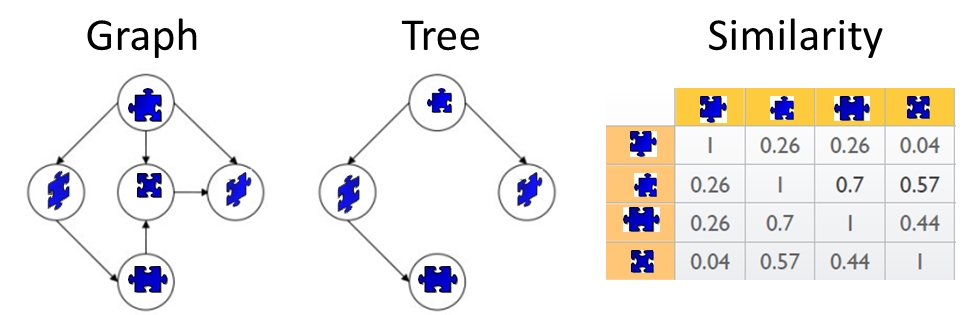
\includegraphics[scale=0.3,trim = 600 0 0 90,clip]{pics/targetrelations}
\end{center} 
Can be done within the framework of vector-valued kernel functions\footnote{Alvarez et al., Kernels for vector-valued functions: a review, Foundation and Trends in Machine Learning, 2012}:
\begin{equation*}
\label{eq:pairwise}
f(\vec{x},\vec{t}) = \vec{w}^T \Psi(\vec{x},\vec{t}) = \sum_{(\bar{\vec{x}},\bar{\vec{t}}) \in \mathcal{D}} \alpha_{(\bar{\vec{x}},\bar{\vec{t}})} \Gamma((\vec{x},\vec{t}),(\bar{\vec{x}},\bar{\vec{t}})) 
\end{equation*}
Model the joint kernel as a product of an instance kernel $k(\cdot,\cdot)$ and a target kernel $g(\cdot,\cdot)$: 
$$\Gamma((\vec{x},\vec{t}),(\bar{\vec{x}},\bar{\vec{t}})) = k(\vec{x},\bar{\vec{x}}) \cdot g(\vec{t},\bar{\vec{t}})$$

\end{frame}

\begin{frame}{Converting graphs to similarities or target representations}

\begin{itemize}
\item {\bf Similarities:} use graph structure to express target similarities
\item[] e.g.\ the shortest-path kernel between two nodes
\item {\bf Representations:}  often characteristics of a specific vertex or edge
\item[] e.g.\ the number of positive labels that are siblings of a vertex\footnote{Rousu et al., Kernel-based learning of hierarchical
multilabel classification models, JMLR 2006} 
\end{itemize}
\begin{center}
\includegraphics[scale=0.4,trim = 0 50 430 0,clip]{Figures/hloss}
\end{center}
\end{frame}

\begin{frame}{A unifying view on MTP methods}

\begin{center}
\includegraphics[scale=0.3]{pics/tools}

\begin{tabular}{ll}
\hline
Group of methods & Applicable setting \\
\hline
\hline
Independent models & B \\
Similarity-enforcing methods & B   \\ 
Relation-exploiting methods & B and D  \\
\alert{Relation-constructing methods} & B \\
Representation-exploiting methods & B and D \\
Representation-constructing methods & A and B \\
\hline  
\end{tabular}
\end{center}
\end{frame}




\begin{frame}{Constructing target hierarchies}

\includegraphics[width=\textwidth]{pics/hierarchies}

\begin{itemize}
\item It might be difficult for a human expert to define a hierarchy\footnote{Rangwala and Naik, Tutorial on Large-Scale Hierarchical Classification, KDD 2017.}
\item Perhaps one can try to learn the hierarchy from data? 
\item Algorithms: level flattening, node removal, hierarchy modification, hierarchy generation, etc.
\end{itemize}


\end{frame}

\begin{frame}[fragile]
\frametitle{Label trees ($\neq$ decision trees) }

\begin{center}
		\vskip3pt
			\tikzset{onslide/.code args={<#1>#2}{%
					\only<#1>{\pgfkeysalso{#2}} % \pgfkeysalso doesn't change the path
				}}
				%\hspace{15pt}
				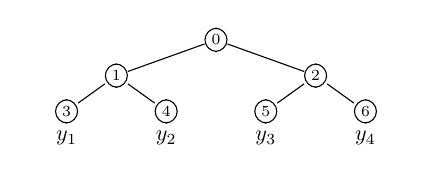
\begin{tikzpicture}[scale = 0.3,every node/.style={scale=0.8},
				regnode/.style={circle,draw,minimum width=1.5ex,inner sep=0pt},
				leaf/.style={circle,fill=black,draw,minimum width=1.5ex,inner sep=0pt},
				pleaf/.style={rectangle,rounded corners=1ex,draw,font=\scriptsize,inner sep=3pt},
				pnode/.style={rectangle,rounded corners=1ex,draw,font=\scriptsize,inner sep=3pt},
				rootnode/.style={rectangle,rounded corners=1ex,draw,font=\scriptsize,inner sep=3pt},
				level/.style={sibling distance=24em/#1, level distance=10ex}
				]
				\node (z) [rootnode] {$0$}
				child {node (a) [pnode] {$1$} 
					child {node [label=below:{\makebox[1cm][c]{$y_1$}}] (b) [pleaf] {3} edge from parent node[above left]{}}
					child {node [label=below:{\makebox[1cm][c]{$y_2$}}] (g) [pleaf] {4} edge from parent node[above right]{}}
					edge from parent node[above left]{}
				}
				child {node (j) [pnode] {$2$}
					child {node [label=below:{\makebox[1cm][c]{$y_3$}}] (k) [pleaf] {5} edge from parent node[above left]{}}
					child {node [label=below:{\makebox[1cm][c]{$y_4$}}] (l) [pleaf] {6}
						{
							child [grow=right] {node (s) {} edge from parent[draw=none]
								child [grow=up] {node (t) {} edge from parent[draw=none]
									child [grow=up] {node (u) {} edge from parent[draw=none]}
								}
							}
						}
						edge from parent node[above right]{}
					}
					edge from parent node[above right]{}
				};
				\end{tikzpicture}
\end{center}
\begin{itemize}
\item Organize classifiers in a tree structure (one leaf $\Leftrightarrow$ one label)
\item Mainly used in multi-class and multi-label classification
\item Goal is fast prediction: almost logarithmic in the number of labels
\item Algorithms: Label embedding trees\footnote{Bengio et al., Label embedding trees for large multi-class tasks, NIPS 2010}, Nested dichotomies\footnote{Frank and Kramer, Ensembles of nested dichotomies for multi-class problems, ICML 2004},
Conditional~probability~trees\footnote{Beygelzimer et al., Conditional probability tree estimation analysis and algorithms. UAI 2009}, Hierarchical softmax\footnote{Morin and Bengio, Hierarchical probabilistic neural network language model, AISTATS 2005}, FastText\footnote{Joulin et al., Bag of tricks for efficient text classifcation. CoRR,
abs/1607.01759, 2016}, Probabilistic classifier chains\footnote{Dembczynski et al., Bayes optimal multilabel classification via probabilistic classifier chains, ICML 2010}%
\end{itemize}
\vskip9pt
\end{frame} 


\begin{frame}
\frametitle{Hierarchical softmax / Probabilistic classifier trees}

\begin{center}
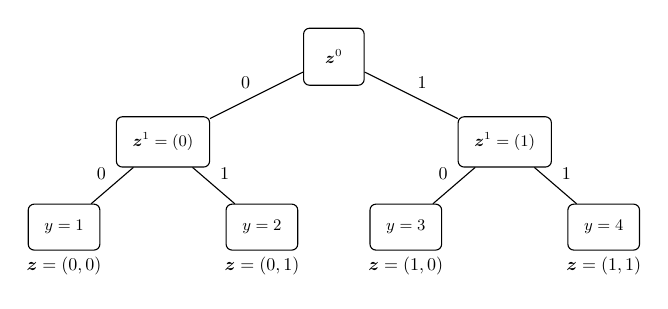
\begin{tikzpicture}[scale = .65,every node/.style={scale=.65},
	regnode/.style={circle,draw,minimum width=1.5ex,inner sep=0pt},
	leaf/.style={circle,fill=black,draw,minimum width=1.5ex,inner sep=9pt},
	pleaf/.style={rectangle,rounded corners=.5ex,draw,font=\small,inner sep=9pt}, %line width=2pt},
	pnode/.style={rectangle,rounded corners=.5ex,draw,font=\small,inner sep=9pt},
	rootnode/.style={rectangle,rounded corners=.5ex,draw,font=\small,inner sep=12pt},
	%level 1/.style={sibling distance=23em, level distance=13ex},
	%level 2/.style={sibling distance=11em, level distance=13ex},
	%regnode/.style={circle,draw,minimum width=1.5ex,inner sep=0pt},
	%leaf/.style={circle,fill=black,draw,minimum width=1.5ex,inner sep=3pt},
	%pleaf/.style={rectangle,rounded corners=.5ex,draw,font=\small,inner sep=3pt},
	%pnode/.style={rectangle,draw,font=\small,inner sep=3pt},
	%rootnode/.style={rectangle,rounded corners=.5ex,draw,font=\small,inner sep=3pt},
	level 1/.style={sibling distance=19em, level distance=11ex},
	level 2/.style={sibling distance=11em, level distance=11ex},
	]
	\node (z) [rootnode] {$\bz^0$}
				child {node (a) [pnode] {$\bz^1 = (0)$} 
					child {node [label=below:{\makebox[1cm][c]{$\bz=(0,0)$}}] (b) [pleaf] {$y=1$} edge from parent node[above left]{$0$}}
					child {node [label=below:{\makebox[1cm][c]{$\bz=(0,1)$}}] (g) [pleaf] {$y=2$} edge from parent node[above right]{$1$}}
					edge from parent node[above left] {$0$}
				}
				child {node (j) [pnode] {$\bz^1 = (1)$}
					child {node [label=below:{\makebox[1cm][c]{$\bz=(1,0)$}}] (k) [pleaf] {$y=3$} edge from parent node[above left]{$0$}}
					child {node [label=below:{\makebox[1cm][c]{$\bz=(1,1)$}}] (l) [pleaf] {$y=4$}
						edge from parent node[above right]{{$1$}}
					}
					edge from parent node[above right]{{$1$}}
				};
\end{tikzpicture}
%\hskip12pt
%\begin{tikzpicture}[scale = .65,every node/.style={scale=.65},
%	regnode/.style={circle,draw,minimum width=1.5ex,inner sep=0pt},
%	leaf/.style={circle,fill=black,draw,minimum width=1.5ex,inner sep=3pt},
%	pleaf/.style={rectangle,rounded corners=.5ex,draw,font=\small,inner sep=3pt},
%	pnode/.style={rectangle,draw,font=\small,inner sep=3pt},
%	rootnode/.style={rectangle,rounded corners=.5ex,draw,font=\small,inner sep=3pt},
%	level 1/.style={sibling distance=13em, level distance=7ex},
%	level 2/.style={sibling distance=9em, level distance=7ex},
%	level 3/.style={sibling distance=9em, level distance=7ex}
%	]
%	\node (z) [rootnode] {$\by^0$}
%				child {node  (a) [label=below:{\makebox[1cm][c]{$\by = (0)$}},pleaf] {$y=1$} 
%					edge from parent node[above left] {$0$}
%				}
%				child {node (j) [pnode] {$\by^1 = (1)$}
%					child {node (b) [pnode] {$\by^2 = (1,0)$}
%					child {node [label=below:{\makebox[1cm][c]{$\by=(1,0,0)$}}] (c) [pleaf] {$y=2$} edge from parent node[above left]{$0$}}
%					child {node [label=below:{\makebox[1cm][c]{$\by=(1,0,1)$}}] (d) [pleaf] {$y=3$} edge from parent node[above right]{$1$}}
%					edge from parent node[above left] {$0$}					
%					}
%					child {node [label=below:{\makebox[1cm][c]{$\by=(1,1)$}}] (l) [pleaf] {$y=4$}
%						edge from parent node[above right]{{$1$}}
%					}
%					edge from parent node[above right]{{$1$}}
%				};
%\end{tikzpicture}
\end{center}
\begin{itemize}
\item Encode the targets by a \emph{prefix code} ($\Rightarrow$ tree structure)\footnote{ Dembczynski et al., Consistency of
probabilistic classifier trees. ECMLPKDD 2016}
\item Multi-class classification: each label $y$ \emph{coded} by $\bz = (z_1, \ldots, z_l) \in \calC$
%\item An internal node identified by a \emph{partial} code $\bz^i = (z_1, \ldots, z_i)$
\item Multi-label classification: a label vector $\by = (y_1, \ldots, y_m)$ is a prefix code.
%\item The code does \emph{not} have to be binary $\Rightarrow$ $b$-ary trees
%\item Different \emph{structures} possible: random tree, Huffman tree, trained structure
\end{itemize}
\end{frame}
%%%%%%%%%%%%%%%%%%%%%%%%%%%%%%%%%%%%%%%%%%%%%%%%%%%%%%%%%%%%%%%%%%%%%%%%%%%%%%% 

%%%%%%%%%%%%%%%%%%%%%%%%%%%%%%%%%%%%%%%%%%%%%%%%%%%%%%%%%%%%%%%%%%%%%%%%%%%%%% 
%\begin{frame}
%\frametitle{Hierarchical softmax (HSM)}
%\begin{itemize}
%\item HSM estimates $\Pr(y\given\bx) $ by following a \emph{path} from the root to a leaf:
%\begin{minipage}[b][1.5cm][c]{\textwidth}
%\only<1>{$$
%\Pr(y \given \bx) = \Pr(\bz \given \bx) = \prod_{i=1}^l \Pr(z_i | {\bz}^{i-1}, \bx)
%$$}
%\only<2>{$$
%\Pr(z_1 \given \bx) \Pr(z_2 \given z_1, \bx) = \frac{\Pr(z_1, \bx)}{\Pr(\bx)}\frac{\Pr(z_2, z_1, \bx)}{\Pr(z_1,\bx)} = \Pr(z_1, z_2 \given \bx)
%$$}
%\end{minipage}
%\begin{center}
%\scalebox{0.9}{%
%\begin{tikzpicture}[scale = 0.65,every node/.style={scale=0.65},
	%regnode/.style={circle,draw,minimum width=1.5ex,inner sep=0pt},
	%leaf/.style={circle,fill=black,draw,minimum width=1.5ex,inner sep=9pt},
	%pleaf/.style={rectangle,rounded corners=.5ex,draw,font=\small,inner sep=9pt}, %line width=2pt},
	%pnode/.style={rectangle,rounded corners=.5ex,draw,font=\small,inner sep=9pt},
	%rootnode/.style={rectangle,rounded corners=.5ex,draw,font=\small,inner sep=12pt},
	%level 1/.style={sibling distance=23em, level distance=13ex},
	%level 2/.style={sibling distance=11em, level distance=13ex},
%]
%\node (z) [rootnode] {$\bx$}
  %child {node (a) [pnode] {$\Pr(z_1=0 \given \bx)=0.4$} 
    %child {node [label=below:{\color{blue}\small \thickmuskip=0mu $\Pr(\bz=(0,0)\given \bx)=0.4$}] (b) [pleaf] {\thickmuskip=-1.5mu $\Pr(z_2=0 \given z_1=0, \bx)=1.0$} edge from parent node[above left]{$z_2=0$}}
    %child {node [label=below:{\small \thickmuskip=0mu $\Pr(\bz=(0,1) \given x)=0.0$}] (g) [pleaf] {\thickmuskip=-1.5mu $\Pr(z_2=1 \given z_1=0, \bx)=0.0$} edge from parent node[above right]{$z_2=1$}}
    %edge from parent node[above left]{$z_1=0$}
  %}
  %child {node (j) [pnode] {$\Pr(z_1=1 \given \bx)=0.6$}
    %child {node [label=below:{ \small \thickmuskip=0mu $\Pr(\bz=(1,0) \given \bx)=0.24$}] (k) [pleaf] {\thickmuskip=-1.5mu $\Pr(z_2=0 \given z_1=1, \bx)=0.4$} edge from parent node[above left]{$z_2=0$}}
      %child {node [label=below:{\color{red} \small \thickmuskip=0mu $\Pr(\bz=(1,1) \given \bx)=0.36$}] (l) [pleaf] {\thickmuskip=-1.5mu $\Pr(z_2=1 \given z_1=1, \bx)=0.6$}
         %{
              %child [grow=right] {node (s) {} edge from parent[draw=none]
                %child [grow=up] {node (t) {} edge from parent[draw=none]
                  %child [grow=up] {node (u) {} edge from parent[draw=none]}
                %}
              %}
        %}
    %edge from parent node[above right]{$z_2=1$}
  %}
  %edge from parent node[above right]{$z_1=1$}
%};
%\end{tikzpicture}
%}%
%\end{center}
%\end{itemize}
%\begin{minipage}[t][3cm][t]{\textwidth}
		%\vskip3pt
			%\begin{itemize}
				%\item Training: \emph{separate} learning problems in the \emph{internal} nodes %($\sum_{z_t} \Pr(z_t \given \bz^{t-1}) = 1$)
				%\item Prediction: \emph{depth first search}/\emph{beam search}
			%\end{itemize}
%\end{minipage}
%\end{frame}
%%%%%%%%%%%%%%%%%%%%%%%%%%%%%%%%%%%%%%%%%%%%%%%%%%%%%%%%%%%%%%%%%%%%%%%%%%%%%%%% 


\begin{frame}
\frametitle{Probabilistic classifier chains}

\begin{itemize}
\item Estimate the {joint} conditional distribution $\Pr(\vec{Y} \given  \vec{x})$. 
\item For optimizing the subset 0/1 loss:  $$ \ell_{0/1}(\by, \hat{\by}) = \assert{\by \ne \hat{\by}}$$
\item Repeatedly apply the \emph{product rule of probability}:
$$
\Pr(\vec{Y} = \vec{y} \given \vec{x}) = \prod_{i=1}^{m} \Pr(Y_i = y_i \given \vec{x}, y_1, \ldots,y_{i-1}) \, .
$$
\item  Learning relies on constructing probabilistic classifiers for estimating 
$$
\Pr(Y_i = y_i|\vec{x}, y_1, \ldots,y_{i-1}) \,,
$$
{independently} for each $i = 1, \ldots, m$. 
%\item One can use scoring functions $f_i(\bx^\prime,y_i)$ and use logistic transformation.
%\item By using the linear models, the overall scoring function takes the form:
%$$
%f(\bx,\by) = \sum_{i=1}^m f_i(\bx, y_i) + \sum_{y_k,y_l} \! f_{k,l}(y_k,y_l) 
%$$
\end{itemize}
\end{frame}

\begin{frame}[fragile]
\begin{itemize}
\item Inference relies on exploiting a probability tree:
\end{itemize}
\vspace{0.1cm}
\begin{center}
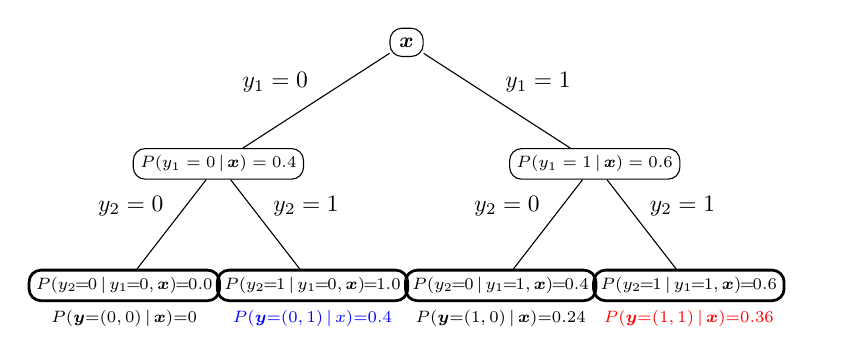
\begin{tikzpicture}[scale = 0.85,every node/.style={scale=0.85},
	regnode/.style={circle,draw,minimum width=1.5ex,inner sep=0pt},
	leaf/.style={circle,fill=black,draw,minimum width=1.5ex,inner sep=0pt},
	pleaf/.style={rectangle,rounded corners=1ex,draw,font=\scriptsize,inner sep=3pt,line width=1pt},
	pnode/.style={rectangle,rounded corners=1ex,draw,font=\scriptsize,inner sep=3pt},
	rootnode/.style={rectangle,rounded corners=1ex,draw,font=\small,inner sep=4pt},
	level/.style={sibling distance=16em/#1, level distance=12ex}
]
\node (z) [rootnode] {$\bx$}
  child {node (a) [pnode] {$P(y_1=0 \given \bx)=0.4$} 
    child {node [label=below:{\scriptsize \thickmuskip=0mu $P(\by=(0,0)\given \bx)=0$}] (b) [pleaf] {\thickmuskip=-1.5mu $P(y_2=0 \given y_1=0, \bx)=0.0$} edge from parent node[above left]{$y_2=0$}}
    child {node [label=below:{\color{blue} \scriptsize \thickmuskip=0mu $P(\by=(0,1) \given x)=0.4$}] (g) [pleaf] {\thickmuskip=-1.5mu $P(y_2=1 \given y_1=0, \bx)=1.0$} edge from parent node[above right]{$y_2=1$}}
    edge from parent node[above left]{$y_1=0$}
  }
  child {node (j) [pnode] {$P(y_1=1 \given \bx)=0.6$}
    child {node [label=below:{\scriptsize \thickmuskip=0mu $P(\by=(1,0) \given \bx)=0.24$}] (k) [pleaf] {\thickmuskip=-1.5mu $P(y_2=0 \given y_1=1, \bx)=0.4$} edge from parent node[above left]{$y_2=0$}}
      child {node [label=below:{\color{red} \scriptsize \thickmuskip=0mu $P(\by=(1,1) \given \bx)=0.36$}] (l) [pleaf] {\thickmuskip=-1.5mu $P(y_2=1 \given y_1=1, \bx)=0.6$}
         {
              child [grow=right] {node (s) {} edge from parent[draw=none]
                child [grow=up] {node (t) {} edge from parent[draw=none]
                  child [grow=up] {node (u) {} edge from parent[draw=none]}
                }
              }
        }
    edge from parent node[above right]{$y_2=1$}
  }
  edge from parent node[above right]{$y_1=1$}
};

%\path (s) -- (t) node [midway] {$\lambda_{2}$};
%\path (t) -- (u) node [midway] {$\lambda_{1}$};
\end{tikzpicture}
\end{center}

\vspace{-0.4cm}
\begin{itemize}
\item For subset 0/1 loss one needs to find $
\bh(\bx) = \argmax_{\by \in \calY} \Pr(\by \given \bx)
$.
\item Greedy and approximate search techniques with guarantees exist.\footnote{Kumar et al., Beam search algorithms for multilabel
learning, Machine Learning 2013}
\item Other losses: compute the prediction on a sample from $\Pr(\vec{Y} \given  \vec{x})$.\footnote{23 Dembczynski et al., An analysis of chaining
in multi-label classification, ECAI 2012}
%\item[]
\end{itemize}

\end{frame}


%\begin{frame}[fragile] 
%\frametitle{Probabilistic classifier chains}
%
%\begin{table}
%\caption{PCC vs. SSVMs on Hamming loss and PCC vs. BR on subset 0/1 loss.%\footnote{\bibentry{Dembczynski_et_al_2012c}\\[1pt]\bibentry{Finley_Joachims_2008}}
%}
%\begin{center}
%\small{\textsc{
%\begin{tabular}{l r@{$\pm$}l r@{$\pm$}l @{$\quad\quad$} r@{$\pm$}l r@{$\pm$}l}
%\toprule
%Dataset & \multicolumn{2}{c}{PCC} & \multicolumn{2}{c@{$\quad\quad$}}{SSVM Best}  & \multicolumn{2}{c}{PCC} & \multicolumn{2}{c}{BR}  \\ 
%&  \multicolumn{4}{c@{$\quad\quad$}}{Hamming loss} & \multicolumn{4}{c}{subset 0/1 loss} \\  
%\midrule
%Scene       &  0.104 &.004  & 0.101&.003 &  0.385&.014  & 0.509&.014\\
%Yeast        &  0.203 &.005 &  0.202&.005  &  0.761&.014 &  0.842&.012\\ 
%Synth1      & 0.067 &.001  & 0.069&.001    & 0.239&.006 & 0.240&.006 \\
%Synth2      & 0.000 &.000  & 0.058&.001  & 0.000&.000  & 0.832&.004 \\
%Reuters     & 0.060 &.002  & 0.045&.001  & 0.598&.009 & 0.689&.008 \\
%Mediamill &  0.172 &.001  & 0.182&.001  &  0.885&.003  & 0.902&.003   \\
%\bottomrule
%\end{tabular}
%}}
%\vspace{0cm}
%\end{center}
%\end{table}
%
%\end{frame}



%
%%%%%%%%%%%%%%%%%%%%%%%%%%%%%%%%%%%%%%%%%%%%%%%%%%%%%%%%%%%%%%%%%%%%%%%%%%%%%%% 
%\begin{frame}
%\frametitle{HSM for MLC}
%\begin{itemize}[<+->]
%\item \emph{Pick-one-label} heuristic used, for example, in \Algo{FastText}:
%$$
%\eta'_j(\bx) = \Pr'(y_j = 1 \given \bx) = \sum_{\by \in \calY} y_j \frac{\Pr(\by \given \bx)}{\sum_{j'=1}^m y_{j'}}
%$$
%\item \emph{Theorem}: inconsistent for label-wise logistic loss and precision$@k$
%\vskip9pt
%%\begin{center}
%\begin{footnotesize}
%\begin{tabular}{c c}
%\toprule
%labels $\by$ & probability $\Pr(\by \given \bx)$ \\
%\midrule
%$\{1\}$ & 0.15 \\
%$\{2\}$ & 0.10 \\
%$\{1, 2\}$ & 0.25 \\
%$\{3\}$ & 0.30 \\
%$\{4\}$ & 0.20 \\
%\bottomrule
%\end{tabular}
%\hskip12pt
%\begin{tabular}{l l}
%\toprule
%True marg. probs & P-o-l marg. probs \\
%\midrule
%$\eta_1(\bx) = 0.4$ & $\eta'_3(\bx) = 0.3$ \\
%$\eta_2(\bx) = 0.35$ & $\eta'_1(\bx) = 0.275$ \\
%$\eta_3(\bx) = 0.3$ & $\eta'_2(\bx) = 0.225$ \\
%$\eta_4(\bx) =0.2$ & $\eta'_4(\bx) =0.2$ \\
%\bottomrule
%& \\
%\end{tabular}
%\end{footnotesize}
%%\end{center}
%\item \vskip9pt \emph{Theorem}: consistent for precision$@k$ for independent labels
%\end{itemize}
%\end{frame}

\begin{frame}{Constructing hierarchies to obtain additional insight}

\begin{itemize}
\item Application in climate science
\item Result of learning 20000 tasks simultaneously with a multi-task learning method
\item Followed by hierarchical clustering of the learned weight vectors\footnote{Papagiannopoulou et al. Globral hydro-climatic biomes identified with multi-task learning, Geoscientific Model Development Discussions 2018}:
\end{itemize}
\begin{center}
\includegraphics[scale=0.2]{Figures/biomes} 
\end{center}

\end{frame}

\begin{frame}{Constructing target similarities by output kernel learning}

\begin{itemize}
\item Consider models $\bf{f}: \mathcal{X} \rightarrow \mathbb{R}^m$
\item Training dataset $\{\bf{x}_i,\bf{y}_i\}_{i=1}^n$
\item Learnable gram matrix $G$ for output kernel $g(\vec{t},\vec{t}')$
\item Learn output kernel and model parameters jointly\footnote{Dinuzzo et al., Learning Output Kernels with Block Coordinate Descent, ICML 2011}:
$$\min_{G \in \mathbb{R}^{m \times m}} \left[ \min_{\bf{f} \in \mathcal{F}} \sum_{i=1}^n \frac{||\bf{f}(\bf{x}_i,\cdot) - \bf{y}_i||_2^2}{2\lambda} + \frac{||\bf{f}||^2_\mathcal{F}}{2} + \frac{
||G||^2_F}{2} \right]$$
\end{itemize}
\begin{center}
\includegraphics[scale=0.2]{Figures/okl}
\end{center}

\end{frame}

\begin{frame}{Constructing decision rules among targets}
\begin{center}
\includegraphics[scale=0.3]{Figures/rules} \\ 
Potential inferred rule\footnote{Loza-Mencia and Janssen, Learning rules for multi-label classification: a stacking and separate-and-conquer approach}: \alert{TEA $\rightarrow$ NOT LEMONADE} \\

\vspace{0.3cm}
\end{center}

\end{frame}


\begin{frame}{A unifying view on MTP methods}

\begin{center}
\includegraphics[scale=0.3]{pics/tools}

\begin{tabular}{ll}
\hline
Group of methods & Applicable setting \\
\hline
\hline
Independent models & B \\
Similarity-enforcing methods & B   \\ 
Relation-exploiting methods & B and D  \\
Relation-constructing methods & B \\
\alert{Representation-exploiting methods} & B and D \\
Representation-constructing methods & A and B \\
\hline  
\end{tabular}
\end{center}
\end{frame}

\begin{frame}{Different learning settings revisited}
   \center
	\vspace{0.4cm}
   \includegraphics[width=0.9\textwidth]{Figures/pictures/Slide16} % requires the graphicx package
\end{frame}

\begin{frame}{An example revisited}
\begin{center}
\includegraphics[width=0.8\textwidth,trim = 0 0 100 30,clip]{Figures/pictures/Slide6}
\end{center}

\end{frame}

%\begin{frame}{Two examples revisited}
%\vspace{0.8cm}
%\includegraphics[width=0.9\textwidth,trim = 0 0 0 90,clip]{Figures/pictures/Slide4}
%
%\end{frame}

\begin{frame}{A target representation in computer vision}

\begin{center}
\includegraphics[scale=0.4]{Figures/semanticclasses} \\
Target representations are the key element of zero-shot learning methods\footnote{Examples taken from the CVPR 2016 Tutorial on Zero-shot learning for Computer Vision} 
\end{center}

\end{frame}

\begin{frame}{Target representations can take many forms}

\begin{center}
\includegraphics[width=\textwidth,trim = 0 0 0 90,clip]{Figures/representations}
\end{center}

\end{frame}

\begin{frame}{Learning target embeddings from text: Word2Vec}

Predict the probability of the next word $w_t$ given the previous words $h$\footnote{Mikolov et al., Efficient Estimation of Word Representations in
Vector Space, Arxiv 2013}:
$$P(w_t \given h) = \frac{\exp(f(w_t,h))}{\sum_{\mathrm{all words}} \exp(f(w_t,h))}$$
\begin{columns}
\begin{column}{5cm}
\includegraphics[scale=0.2]{Figures/word2vec}
\end{column}
\begin{column}{6cm}
\hspace{1cm} \includegraphics[scale=0.2]{Figures/kingqueen}
\end{column}
\end{columns}



\end{frame}

\begin{frame}{Different learning settings revisited}
   \center
	\vspace{0.4cm}
   \includegraphics[width=0.9\textwidth]{Figures/pictures/Slide16} % requires the graphicx package
\end{frame}

\begin{frame}{Kronecker kernel ridge regression}

\vspace{0.5cm}
Pairwise model representation in the primal: 
\begin{equation*}
\label{eq:pairwise}
f(\vec{x},\vec{t}) = \vec{w}^T \left(\phi(\vec{x}) \otimes \psi(\vec{t}) \right) 
\end{equation*}
Kronecker product pairwise kernel in the dual\footnote{Stock et al., A comparative study of pairwise learning methods based on kernel ridge regression, Neural Computation 2018}:
\begin{eqnarray*} 
f(\vec{x},\vec{t})= \sum_{(\bar{\vec{x}},\bar{\vec{t}}) \in \mathcal{D}} \alpha_{(\bar{\vec{x}},\bar{\vec{t}})}  k(\vec{x},\bar{\vec{x}}) \cdot g(\vec{t},\bar{\vec{t}})  = \sum_{(\bar{\vec{x}},\bar{\vec{t}}) \in \mathcal{D}} \alpha_{(\bar{\vec{x}},\bar{\vec{t}})} \Gamma((\vec{x},\vec{t}),(\bar{\vec{x}},\bar{\vec{t}})) 
\end{eqnarray*}
Least-squares minimization with 
$\bm{z} = \textrm{vec}{(Y)}$: 
$$ \min_{\bm{\boldsymbol\alpha}} \, ||\bm{\kkernelm}\bm{\boldsymbol\alpha} -\bm{z} ||^2_2 +\regparam\bm{\boldsymbol\alpha }\transpose\kkernelm\bm{\boldsymbol\alpha} $$


\end{frame}

%
%\begin{frame}{Two-step zero-shot learning\footnote{Pahikkala et al. A two-step approach for solving full and almost full cold-start problems in dyadic prediction, ECML/PKDD 2014.} \footnote{Romero-Paredes and Torr, An embarrassingly simple approach to zero-shot learning, ICML 2015.}}
%\begin{columns}[c]
%\column{0.6\textwidth}
  %\center 
   %\includegraphics[width=0.7\textheight]{Figures/concept2SRLS}
%
%\column{0.4\textwidth}
%\begin{enumerate}
%\item Build a kernel ridge regression model to generalize to \alert{new instances}
%\item Build a kernel ridge regression model to generalize to \alert{new tasks}
%\end{enumerate}
%\end{columns}
%\end{frame}

\begin{frame}{Two-step zero-shot learning\footnote{Pahikkala et al. A two-step approach for solving full and almost full cold-start problems in dyadic prediction, ECML/PKDD 2014.} \footnote{Romero-Paredes and Torr, An embarrassingly simple approach to zero-shot learning, ICML 2015.}}
% voorbeeldje met boeken
\vspace{0.5cm}
\includegraphics[width=0.75\textwidth,trim = 0 0 0 90,clip]{Figures/pictures/Slide8}
\end{frame}


\begin{frame}{Two-step zero-shot learning\footnote{Pahikkala et al. A two-step approach for solving full and almost full cold-start problems in dyadic prediction, ECML/PKDD 2014.} \footnote{Romero-Paredes and Torr, An embarrassingly simple approach to zero-shot learning, ICML 2015.}}
% voorbeeldje met boeken
\vspace{0.5cm}
\includegraphics[width=0.75\textwidth,trim = 0 0 0 90,clip]{Figures/pictures/Slide9}
\end{frame}

\begin{frame}{Two-step zero-shot learning\footnote{Pahikkala et al. A two-step approach for solving full and almost full cold-start problems in dyadic prediction, ECML/PKDD 2014.} \footnote{Romero-Paredes and Torr, An embarrassingly simple approach to zero-shot learning, ICML 2015.}}
% voorbeeldje met boeken
\vspace{0.5cm}
\includegraphics[width=0.75\textwidth,trim = 0 0 0 90,clip]{Figures/pictures/Slide10}
\end{frame}

%\begin{frame}{Two-step kernel ridge regression}
%
%\vspace{0.6cm}
%\begin{itemize}
%\item Kernel evaluations for new test instance: 
%$$\bm{k}(\bm{x})=\left(\kernelf(\bm{x},\bm{x}_1),\ldots,\kernelf(\bm{x},\bm{x}_\osize)\right)\transpose$$ 
%$$\bm{g}(\bm{t})=\left(\gkernelf(\bm{t},\bm{t}_1),\ldots,\gkernelf(\bm{t},\bm{t}_m)\right)\transpose$$ \pause 
%\item Step 1: prediction for $\bm{x}$ on all the training targets
%$$
%\mathbf{\predfun}_\taskset (\bm{x}) = \bm{k}(\bm{x})\transpose A^{IT} = \bm{k}(\bm{x})\transpose \left(\dkernelm+\regparam_1 \idmatrix\right)^{-1} Y  $$ \pause 
%\item Step 2: generalizing to new targets
%\begin{eqnarray*}
%\predfun^\text{TS}(\bm{x}, \bm{t}) &=&  \bm{g}(\bm{t})\transpose \left(\tkernelm+\regparam_2 \idmatrix\right)^{-1}  \mathbf{\predfun}_\taskset (\bm{x})\transpose \\ \pause 
%&=& \bm{k}(\bm{x})\transpose \left(\dkernelm+\regparam_1 \idmatrix\right)^{-1} Y  \left(\tkernelm+\regparam_2 \idmatrix\right)^{-1} \bm{g}(\bm{t}) \\ \pause 
%&=& \bm{k}(\bm{x})\transpose A^\text{TS} \bm{g}(\bm{t}) \\
%&=& \vec{w}^T \left(\phi(\vec{x}) \otimes \psi(\vec{t}) \right)
%\end{eqnarray*}
%\end{itemize}
%\end{frame}


%
%\begin{frame}{Almost zero-shot learning: \\
%definition and experimental setup}
 %\center
%
   %\includegraphics[width=\textwidth]{Figures/relationMatrices} \\
	%
	%Gradually increase the number of training instances for the ``new" task 
%\end{frame}
%
%\begin{frame}{Almost zero-shot learning: \\
%results for protein-ligand interaction prediction}
 %\center
   %\includegraphics[width=\textwidth]{Figures/results4} \\
%\end{frame}


\begin{frame}{Zero-shot learning in computer vision}

\begin{center}
\includegraphics[width=0.75\textwidth]{Figures/zero-shot}
\end{center}

\end{frame}

\begin{frame}{Zero-shot learning in computer vision}

\vspace{0.5cm}
Pairwise model representation as before: 
\begin{equation*}
\label{eq:pairwise}
f(\vec{x},\vec{t}) = \vec{w}^T \left(\phi(\vec{x}) \otimes \psi(\vec{t}) \right) 
\end{equation*}
Inference in a structured prediction fashion: 
$$\hat{c}(\vec{x}) = \argmax_{\vec{t} \in \mathcal{T}} f(\vec{x},\vec{t})$$
Different optimization problems: 
\begin{itemize}
\item Multi-class objective\footnote{Akata et al., Evaluation of Output Embeddings for Fine-Grained Image Classification, CVPR2015}
\item Ranking objective\footnote{Frome et al., Devise: A deep visual-semantic embedding
model, NIPS 2013}
\item Regression objective\footnote{Socher et al., g. Zero-shot learning through cross-modal transfer, NIPS 2013}
\item Canonical correlation analysis
\end{itemize}
Different model formulations: 
\begin{itemize}
\item Linear embeddings
\item Nonlinear embeddings
\end{itemize}
\vspace{0.3cm}
\end{frame}


\begin{frame}

\begin{center}
\includegraphics[scale=0.5]{Figures/interaction}
\end{center}
\begin{exampleblock}{Question}
In which situation(s) is it useful to exploit target relations and representations?   
\begin{itemize}
\item In Setting B, when $n$ is sufficiently large
\item In Setting B, when $n$ is sufficiently small
\item In Setting D, when $n$ is sufficiently large
\item In Setting D, when $n$ is sufficiently small
\end{itemize}
\end{exampleblock}
\end{frame}


\begin{frame}{A case study on the Wikipedia dataset}
\begin{center}
\includegraphics[width=0.75\textwidth,trim = 0 0 100 0,clip]{Figures/pictures/Slide5}
\end{center}
\end{frame}



\begin{frame}{The answer}  
 \center

\vspace{-0.5cm}
   \includegraphics[width=0.65\textwidth]{Figures/lc_wiki} \\
   $12,000$ labels: from $5,000$ to $350,000$ instances\footnote{M. Stock, Exact and efficient algorithms for pairwise learning, PhD thesis, 2017}
	\vspace{0.2cm}
\end{frame}


\begin{frame}{A unifying view on MTP methods}

\begin{center}
\includegraphics[scale=0.3]{pics/tools}

\begin{tabular}{ll}
\hline
Group of methods & Applicable setting \\
\hline
\hline
Independent models & B \\
Similarity-enforcing methods & B   \\ 
Relation-exploiting methods & B and D  \\
Relation-constructing methods & B \\
Representation-exploiting methods & B and D \\
\alert{Representation-constructing methods} & A and B \\
\hline  
\end{tabular}
\end{center}
\end{frame}

\begin{frame}{Different learning settings revisited}
   \center
	\vspace{0.4cm}
   \includegraphics[width=0.9\textwidth]{Figures/pictures/Slide16} % requires the graphicx package
\end{frame}


\begin{frame}{Low-rank approximation in Settings B and C}

\begin{center}
\includegraphics[width=9cm]{pics/lowrank}
\end{center}
Typically perform a low-rank approximation of the parameter matrix\footnote{Chen et al., A convex formulation for learning shared structures from
multiple tasks, ICML 2009. }:
$$\min_A ||Y - XA ||^2_F + \lambda \, \mathrm{rank}(A)$$

\end{frame}



%%%%%%%%%%%%%%%%%%%%%%%%%%%%%%%%%%%%%%%%%%%%%%%%%%%%%%%%%%%%%%%%%%%%%%%%%%%%%% 
%%%%%%%%%%%%%%%%%%%%%%%%%%%%%%%%%%%%%%%%%%%%%%%%%%%%%%%%%%%%%%%%%%%%%%%%%%%%%%  

%%%%%%%%%%%%%%%%%%%%%%%%%%%%%%%%%%%%%%%%%%%%%%%%%%%%%%%%%%%%%%%%%%%%%%%%%%%%%% 
%%%%%%%%%%%%%%%%%%%%%%%%%%%%%%%%%%%%%%%%%%%%%%%%%%%%%%%%%%%%%%%%%%%%%%%%%%%%%% 
\frame{
  \frametitle{Low-rank approximation in Settings B and C}
  


\begin{itemize}
 \item $A$: parameter matrix of dimensionality $p \times m$ 
\item $p$: the number of features
\item $m$: the number of targets
\item Assume a low-rank structure of $A$:

\begin{center}
$$  U \qquad \qquad \times \qquad  V \qquad \qquad  =  \qquad  A$$

\includegraphics[width=0.75\textwidth,trim = 0 0 0 0,clip]{Figures/nmf2}

%\begin{columns}
%\column{0.45\columnwidth}
%\centering
%$
%\begin{bmatrix}
%\rule[.5ex]{4.5em}{0.4pt}\vec{a}_1 \rule[.5ex]{4.5em}{0.4pt}\\
%\rule[.5ex]{4.5em}{0.4pt}\vec{a}_2 \rule[.5ex]{4.5em}{0.4pt}\\
%\vdots \\
%\rule[.5ex]{4.5em}{0.4pt}\vec{a}_n \rule[.5ex]{4.5em}{0.4pt}\\
%\end{bmatrix}_{p\times m} \Rightarrow
%$ 
%
%\column{0.35\columnwidth}
%$
%\begin{bmatrix}
%\rule[.5ex]{1.5em}{0.4pt}\vec{z}_1 \rule[.5ex]{1.5em}{0.4pt}\\
%\rule[.5ex]{1.5em}{0.4pt}\vec{z}_2 \rule[.5ex]{1.5em}{0.4pt}\\
%\vdots \\
%\rule[.5ex]{1.5em}{0.4pt}\vec{z}_n \rule[.5ex]{1.5em}{0.4pt}\\
%\end{bmatrix}_{p\times \hat{m}}
%\hspace{-0.2in}
%$
%\end{columns}
\end{center}

\item We can write $A=VU$ and $A \vec{x} = VU \vec{x}$
\item $V$ is a $p \times \hat{m}$ matrix
\item  $U$ i an $\hat{m} \times m$ matrix

\item $\hat{m}$ is the rank of $A$

\end{itemize}

}

\begin{frame}{Low-rank approximation in Settings B and C}{Overview of methods}

\begin{itemize}
\item Popular for multi-output regression, multi-task learning and multi-label classification
\item Linear as well as nonlinear methods
\item Algorithms: 
\begin{itemize}
\item Principal component analysis\footnote{Weston et al., Kernel dependency estimation, NIPS 2002}, Canonical correlation analysis\footnote{Multi-label prediction via sparse infinite CCA, NIPS 2009}, Partial least squares
\item Singular value decomposition\footnote{Tai and Lin, Multilabel classification with principal label space transformation, Neural Computation 2012}, Alternating structure optimization\footnote{Zhou et al., Clustered Multi-Task Learning Via Alternating Structure Optimization, NIPS 2011}
\item Compressed sensing\footnote{Hsu et al., Multi-label prediction via compressed sensing. NIPS 2009}, Output codes\footnote{Zhang and Schneider, Multi-label Output Codes using Canonical Correlation Analysis, UAI 2011}, Landmark labels\footnote{Balasubramanian and Lebanon, The landmark selection method for multiple output
prediction, ICML 2012}, Bloom filters\footnote{Ciss\'e et al., Robust bloom filters for large multilabel
classification tasks, NIPS 2013}, Auto-encoders\footnote{Wicker et al., A nonlinear label compression and transformation
method for multi-label classification using autoencoders, PAKDD 2016}
\end{itemize}
\end{itemize}
\vspace{0.3cm}
\end{frame}

%%%%%%%%%%%%%%%%%%%%%%%%%%%%%%%%%%%%%%%%%%%%%%%%%%%%%%%%%%%%%%%%%%%%%%%%%%%%%% 
%%%%%%%%%%%%%%%%%%%%%%%%%%%%%%%%%%%%%%%%%%%%%%%%%%%%%%%%%%%%%%%%%%%%%%%%%%%%%% 

%%%%%%%%%%%%%%%%%%%%%%%%%%%%%%%%%%%%%%%%%%%%%%%%%%%%%%%%%%%%%%%%%%%%%%%%%%%%%% 
%%%%%%%%%%%%%%%%%%%%%%%%%%%%%%%%%%%%%%%%%%%%%%%%%%%%%%%%%%%%%%%%%%%%%%%%%%%%%% 
%\frame{
  %\frametitle{\normalsize Low-dimensional Label Embeddings}
%
%\begin{itemize}
%
%\item Otherwise, we may directly map the input $\vec{x}$ to its corresponding prediction $\hat{\vec{y}} = \vec{U}^{\dagger}\vec{V}\vec{x}$ 
%\item Here $\vec{U}^{\dagger}$ is the decompression matrix which lifts intermediary prediction $\vec{V}\vec{x}$ from the embedding space to original label space \pause
%
%\end{itemize}
%
%\begin{columns}
%\column{0.30\columnwidth}
%\centering
%$
%\begin{bmatrix}
%\rule[.5ex]{2.0em}{0.4pt}\vec{x}_1 \rule[.5ex]{2.0em}{0.4pt}\\
%\rule[.5ex]{2.0em}{0.4pt}\vec{x}_2 \rule[.5ex]{2.0em}{0.4pt}\\
%\vdots \\
%\rule[.5ex]{2.0em}{0.4pt}\vec{x}_n \rule[.5ex]{2.0em}{0.4pt}\\
%\end{bmatrix}_{n\times d}
%\Rightarrow{\vec{V}}\hspace{-0.3in}
%$
%\column{0.30\columnwidth}
%\centering
%$
%\hspace{-0.3in}
%\begin{bmatrix}
%\rule[.5ex]{1.5em}{0.4pt}\vec{z}_1 \rule[.5ex]{1.5em}{0.4pt}\\
%\rule[.5ex]{1.5em}{0.4pt}\vec{z}_2 \rule[.5ex]{1.5em}{0.4pt}\\
%\vdots \\
%\rule[.5ex]{1.5em}{0.4pt}\vec{z}_n \rule[.5ex]{1.5em}{0.4pt}\\
%\end{bmatrix}_{n\times \hat{m}}
%\Rightarrow{\vec{U}^{\dagger}}\hspace{-0.3in}
%$
%\column{0.40\columnwidth}
%$
%\begin{bmatrix}
%\rule[.5ex]{3.5em}{0.4pt}\vec{y}_1 \rule[.5ex]{3.5em}{0.4pt}\\
%\rule[.5ex]{3.5em}{0.4pt}\vec{y}_2 \rule[.5ex]{3.5em}{0.4pt}\\
%\vdots \\
%\rule[.5ex]{3.5em}{0.4pt}\vec{y}_n \rule[.5ex]{3.5em}{0.4pt}\\
%\end{bmatrix}_{n\times m}
%$ 
%
%\end{columns}
%
%}
%
%%%%%%%%%%%%%%%%%%%%%%%%%%%%%%%%%%%%%%%%%%%%%%%%%%%%%%%%%%%%%%%%%%%%%%%%%%%%%%% 
%%%%%%%%%%%%%%%%%%%%%%%%%%%%%%%%%%%%%%%%%%%%%%%%%%%%%%%%%%%%%%%%%%%%%%%%%%%%%%% 
%\frame{
  %\frametitle{\normalsize Label Embedding Methods}
%
%Various methods differ in terms of the embedding/compression and de-compression methods they employ
%
%\begin{itemize}
 %\item  Methods for label embedding
	%\begin{itemize}
		 	%\item Compressed Sensing \footnote{\bibentry{Hsu_et_al_2009}}
 		%\item Label Embedding for Missing Labels (LEML) \footnote{\bibentry{Yu_et_al_2014}}
 		%\item Sparse Local Embeddings for Extreme Classification (SLEEC) 			\footnote{\bibentry{Bhatia_etal_2015}}
 	%\end{itemize}
 %
%\end{itemize}
%}

\frame{
  \frametitle{Target embeddings in neural networks}
  
  %\begin{columns}
%\column{0.40\columnwidth}
%\begin{itemize}
%\item Shallow Networks - SVM
	%\begin{itemize}
	%\vspace{-0.2in}
		%\item Direct mapping of input to output
	%\end{itemize}
%\end{itemize}
%\centering
%
\tikzset{%
  every neuron/.style={
    circle,
    draw,
    minimum size=1.0cm
  },
  neuron missing/.style={
    draw=none, 
    scale=4,
    text height=0.333cm,
    execute at begin node=\color{black}$\vdots$
  },===
}
\scalebox{0.4}{
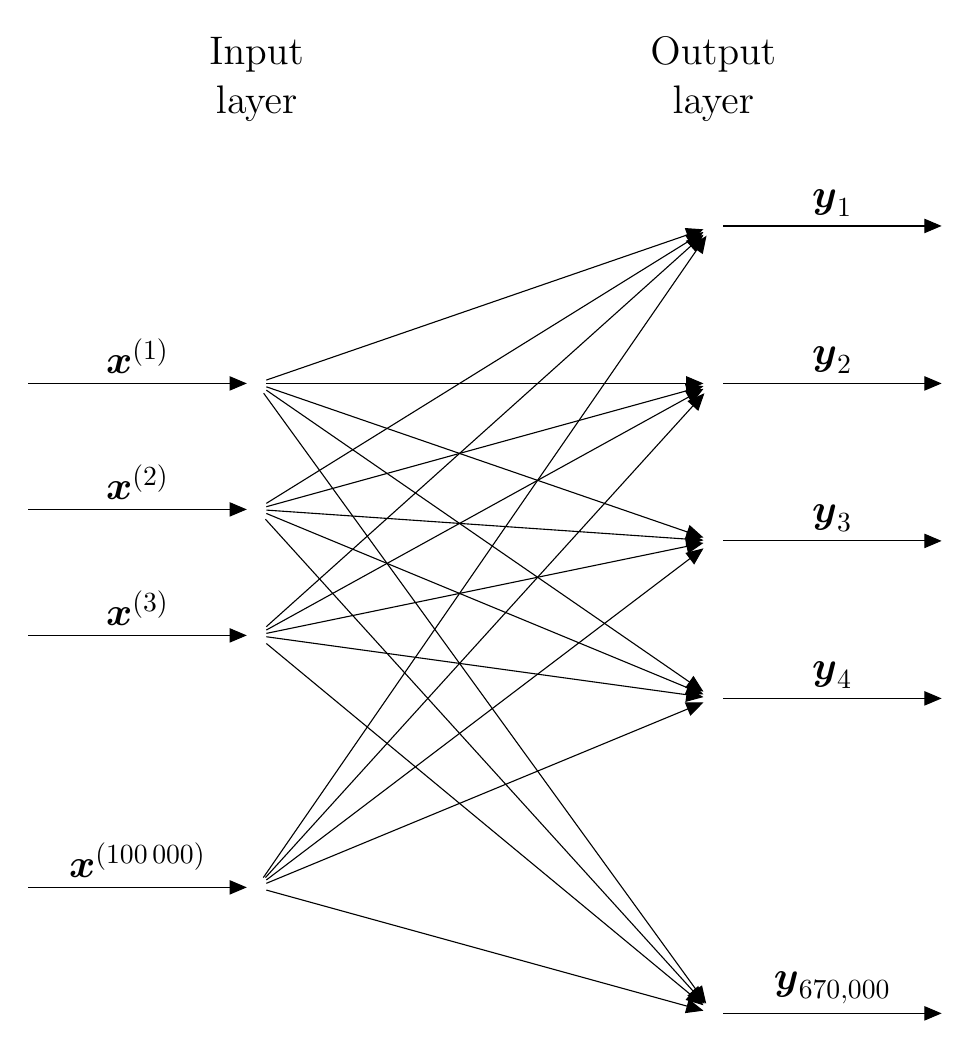
\begin{tikzpicture}[x=2.9cm, y=1.6cm, >=stealth, font=\Large]

\foreach \m/\l [count=\y] in {1,2,3,missing,4}
  \node [every neuron/.try, neuron \m/.try] (input-\m) at (0,2.5-\y) {};

\foreach \m [count=\y] in {1,2,3,4,missing,5}
  \node [every neuron/.try, neuron \m/.try ] (hidden-\m) at (2,4.0-\y*1.25) {};



%\foreach \m [count=\y] in {1,missing,2}
%  \node [every neuron/.try, neuron \m/.try ] (output-\m) at (4,1.5-\y) {};

\foreach \l [count=\i] in {1,2,3,100\,000}
  \draw [style={<-,>=triangle 45}] (input-\i) -- ++(-1,0)
    node [above, midway] {$\vec{x}^{(\l)}$};


%\foreach \l [count=\i] in {1,2}
%  \draw [->] (hidden-\i) -- ++(1,0)
%    node [above, midway] {$O_\l$};
    
    \draw [style={->,>=triangle 45}]  (hidden-1) -- ++(1,0)
    node [above, midway] {$\vec{y}_1$};
    
    \draw [style={->,>=triangle 45}]  (hidden-2) -- ++(1,0)
    node [above, midway] {$\vec{y}_{2}$};
    
    \draw [style={->,>=triangle 45}]  (hidden-3) -- ++(1,0)
    node [above, midway] {$\vec{y}_{3}$};
    
    \draw [style={->,>=triangle 45}]  (hidden-4) -- ++(1,0)
    node [above, midway] {$\vec{y}_{4}$};
    
    \draw [style={->,>=triangle 45}]  (hidden-5) -- ++(1,0)
    node [above, midway] {$\vec{y}_{670,000}$};
    
%\foreach \l [count=\i] in {1}
%  \node [above] at (hidden-1.north) {$O_1$};
%	\node [above] at (hidden-2.north) {$O_{670\,000}$};
	
  
%\foreach \l [count=\i] in {1,2}
%  \draw [->] (hidden-\i) -- ++(1,0)
%    node [above, midway] {$O_\l$};

\foreach \i in {1,...,4}
  \foreach \j in {1,...,5}
    \draw [style={->,>=triangle 45}] (input-\i) -- (hidden-\j);

    
%    \foreach \i in {1,...,3}
%  \foreach \j in {1,...,2}
%    \draw [style={->,>=triangle 45}] (input-\i) -- (hidden-\j)
%    node [above, midway] {$\textbf{W}_{(\i,\j)}$};

%    \draw [style={->,>=triangle 45}] (input-1) -- (hidden-1)
%    node [above, midway] {$\textbf{W}_{(1,1)}$};
%    
%    \draw [style={->,>=triangle 45}] (input-2) -- (hidden-1)
%    node [above, midway] {$\textbf{W}_{(2,1)}$};
%    
%    \draw [style={->,>=triangle 45}] (input-3) -- (hidden-1)
%    node [above, midway] {$\textbf{W}_{(3,1)}$};
%    
%    \draw [style={->,>=triangle 45}] (input-4) -- (hidden-1)
%    node [below, near start] {$\textbf{W}_{(51033,1)}$};
    
%    \draw [style={->,>=triangle 45}] (input-1) -- (hidden-2)
%    node [above, midway] {$\textbf{W}_{(1,2)}$};
    
%    \draw [style={->,>=triangle 45}] (input-1) -- (hidden-1)
%    node [above, midway] {$\textbf{W}_{(1,1)}$};
%    
%    \draw [style={->,>=triangle 45}] (input-1) -- (hidden-1)
%    node [above, midway] {$\textbf{W}_{(1,1)}$};  

%\foreach \i in {1,...,2}
%  \foreach \j in {1,...,2}
%    \draw [->] (hidden-\i) -- (output-\j);

\foreach \l [count=\x from 0] in {Input, Output}
  \node [align=center, above] at (\x*2,3.5) {\l \\ layer};
 

\end{tikzpicture}}\pause
%\column{0.45\columnwidth}
%\begin{itemize}
%\vspace{-0.10in}
%\item Label embedding 

%\end{itemize}
\begin{center}
\begin{huge}

\tikzset{%
  every neuron/.style={
    circle,
    draw,
    minimum size=1.0cm
  },
  neuron missing/.style={
    draw=none, 
    scale=4,
    text height=0.333cm,
    execute at begin node=\color{black}$\vdots$
  },===
}
\scalebox{0.35}{
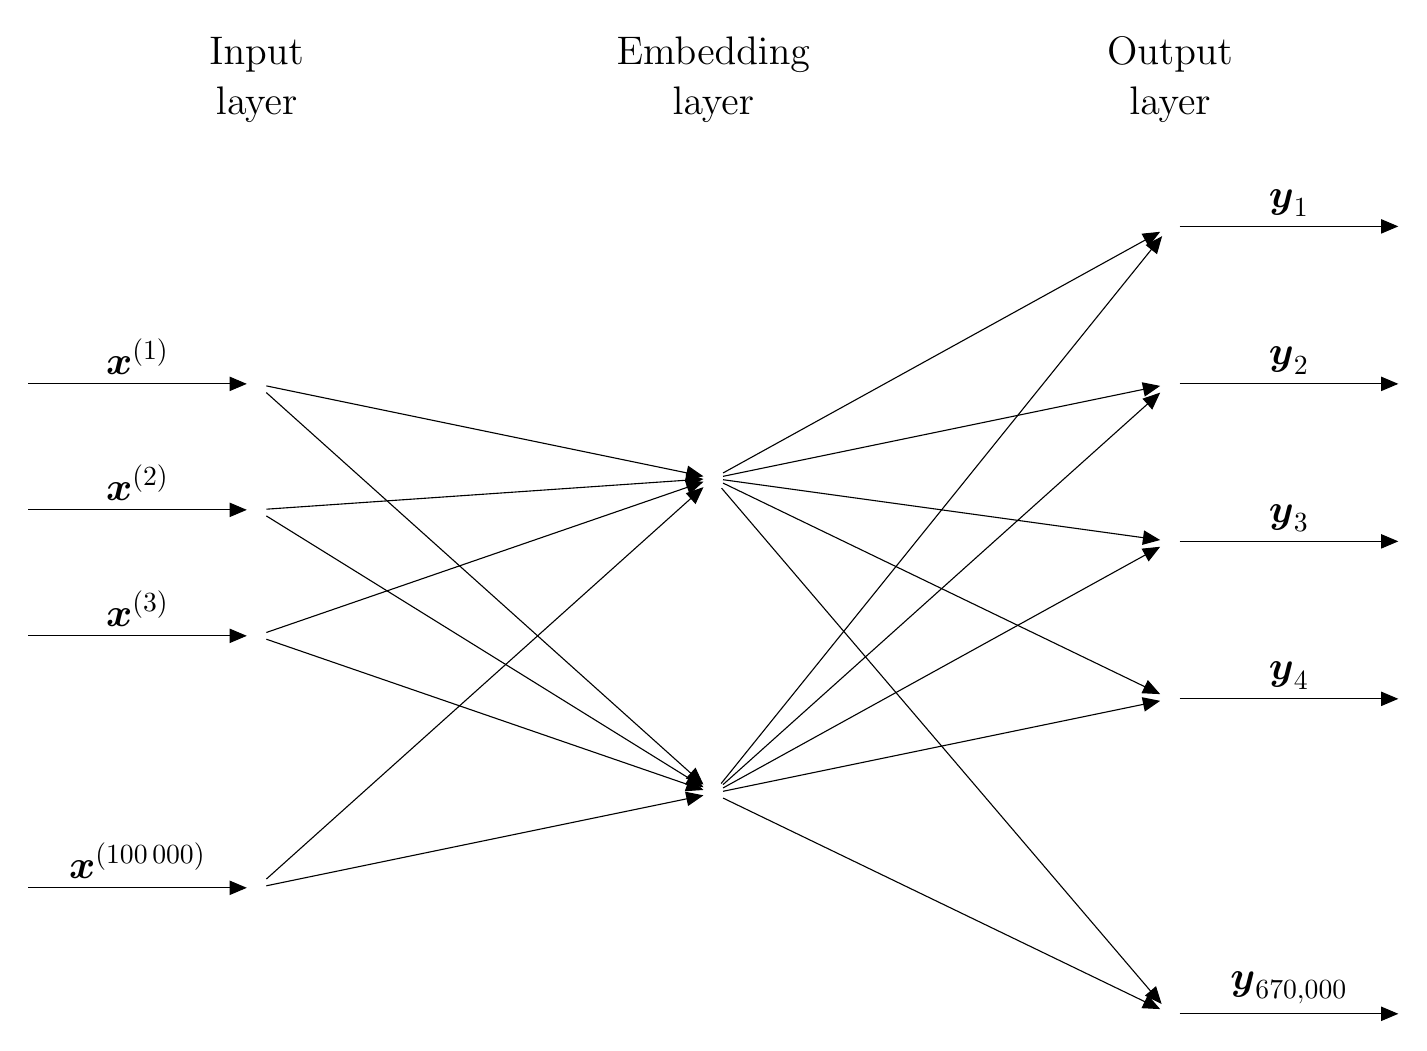
\begin{tikzpicture}[x=2.9cm, y=1.6cm, >=stealth, font=\Large]

\foreach \m/\l [count=\y] in {1,2,3,missing,4}
  \node [every neuron/.try, neuron \m/.try] (input-\m) at (0,2.5-\y) {};
  
\foreach \m [count=\y] in {1,missing,2}
  \node [every neuron/.try, neuron \m/.try ] (hidden1-\m) at (2,2.0-\y*1.25) {};

\foreach \m [count=\y] in {1,2,3,4,missing,5}
  \node [every neuron/.try, neuron \m/.try ] (hidden-\m) at (4,4.0-\y*1.25) {};



%\foreach \m [count=\y] in {1,missing,2}
%  \node [every neuron/.try, neuron \m/.try ] (output-\m) at (4,1.5-\y) {};

\foreach \l [count=\i] in {1,2,3,100\,000}
  \draw [style={<-,>=triangle 45}] (input-\i) -- ++(-1,0)
    node [above, midway] {$\vec{x}^{(\l)}$};


%  \draw [style={->,>=triangle 45}]  (hidden1-1) -- ++(1,0)
%    node [above, midway] {$\textbf{H}_1$};
%    
%  \draw [style={->,>=triangle 45}]  (hidden1-2) -- ++(1,0)
%    node [above, midway] {$\textbf{H}_2$};
    
%\foreach \l [count=\i] in {1,2}
%  \draw [->] (hidden-\i) -- ++(1,0)
%    node [above, midway] {$O_\l$};
    
    \draw [style={->,>=triangle 45}]  (hidden-1) -- ++(1,0)
    node [above, midway] {$\vec{y}_1$};
    
    \draw [style={->,>=triangle 45}]  (hidden-2) -- ++(1,0)
    node [above, midway] {$\vec{y}_{2}$};
    
    \draw [style={->,>=triangle 45}]  (hidden-3) -- ++(1,0)
    node [above, midway] {$\vec{y}_{3}$};
    
    \draw [style={->,>=triangle 45}]  (hidden-4) -- ++(1,0)
    node [above, midway] {$\vec{y}_{4}$};
    
    \draw [style={->,>=triangle 45}]  (hidden-5) -- ++(1,0)
    node [above, midway] {$\vec{y}_{670,000}$};
    
%\foreach \l [count=\i] in {1}
%  \node [above] at (hidden-1.north) {$O_1$};
%	\node [above] at (hidden-2.north) {$O_{670\,000}$};
	
  
%\foreach \l [count=\i] in {1,2}
%  \draw [->] (hidden-\i) -- ++(1,0)
%    node [above, midway] {$O_\l$};

\foreach \i in {1,...,4}
  \foreach \j in {1,...,2}
    \draw [style={->,>=triangle 45}] (input-\i) -- (hidden1-\j);
    
\foreach \i in {1,...,2}
  \foreach \j in {1,...,5}
    \draw [style={->,>=triangle 45}] (hidden1-\i) -- (hidden-\j);

    
%    \foreach \i in {1,...,3}
%  \foreach \j in {1,...,2}
%    \draw [style={->,>=triangle 45}] (input-\i) -- (hidden-\j)
%    node [above, midway] {$\textbf{W}_{(\i,\j)}$};

%    \draw [style={->,>=triangle 45}] (input-1) -- (hidden-1)
%    node [above, midway] {$\textbf{W}_{(1,1)}$};
%    
%    \draw [style={->,>=triangle 45}] (input-2) -- (hidden-1)
%    node [above, midway] {$\textbf{W}_{(2,1)}$};
%    
%    \draw [style={->,>=triangle 45}] (input-3) -- (hidden-1)
%    node [above, midway] {$\textbf{W}_{(3,1)}$};
%    
%    \draw [style={->,>=triangle 45}] (input-4) -- (hidden-1)
%    node [below, near start] {$\textbf{W}_{(51033,1)}$};
    
%    \draw [style={->,>=triangle 45}] (input-1) -- (hidden-2)
%    node [above, midway] {$\textbf{W}_{(1,2)}$};
    
%    \draw [style={->,>=triangle 45}] (input-1) -- (hidden-1)
%    node [above, midway] {$\textbf{W}_{(1,1)}$};
%    
%    \draw [style={->,>=triangle 45}] (input-1) -- (hidden-1)
%    node [above, midway] {$\textbf{W}_{(1,1)}$};  

%\foreach \i in {1,...,2}
%  \foreach \j in {1,...,2}
%    \draw [->] (hidden-\i) -- (output-\j);

\foreach \l [count=\x from 0] in {Input, Embedding, Output}
  \node [align=center, above] at (\x*2,3.5) {\l \\ layer};
 

\end{tikzpicture}}
\end{huge}
\end{center}
%\end{columns}
\begin{itemize}
	\item Mapping input to output via embedding layer
	\item Nonlinear alternative to $A\vec{x} = VU \vec{x}$
\end{itemize}
}


\begin{frame}{Low-rank approximation in Setting A}

Factorize the matrix $Y$ instead of the parameter matrix $A$: 
\begin{center}
\includegraphics[width=11cm]{Figures/matrixcompletion2}
\end{center}
$$Y \qquad = \qquad  U \qquad \times \qquad V \qquad $$

\end{frame}

\begin{frame}{Low-rank approximation in Setting A}
{Overview of algorithms}

\begin{itemize}
\item Nuclear norm minimizationan\footnote{Candes and Recht, Exact low-rank matrix completion via convex optimization. Foundations
of Computational Mathematics 2008}
\item Gaussian processes\footnote{Lawrence and Urtasun, Non-linear matrix factorization with Gaussian processes, ICML 2009}
\item Probabilistic methods\footnote{Shan and Banerjee, Generalized probabilistic matrix factorizations for collaborative
filtering, ICDM 2010} 
\item Spectral regularization\footnote{Mazumder et al., Spectral regularization algorithms for learning large incomplete matrices., JMLR 2010} 
\item Non-negative matrix factorization\footnote{Gaujoux and Seoighe, A flexible R package for nonnegative matrix factorization.
BMC bioinformatics 2010}
\item Alternating least-squares minimization\footnote{Jain et al., Low-rank matrix completion using alternating minimization, ACM Symposium on Theory of Computing 2013}
\end{itemize}

\end{frame}

\begin{frame}{Matrix factorization with side information for Setting A}

\begin{center}
\includegraphics[scale=0.3]{pics/settingA}
\end{center}
\begin{itemize}
\item Construct \alert{implicit} features $(\vec{x}^I,\vec{t}^I)$ for users and items with matrix factorization methods
\item Exploit \alert{explicit} features $(\vec{x}^E,\vec{t}^E)$ (a.k.a. side information)
\item Concatenate: 
$$\vec{x}^C = (\vec{x}^I,\vec{x}^E), \qquad \vec{t}^C = (\vec{t}^I,\vec{t}^E)$$
\item Apply methods that we have seen before\footnote{Menon and Elkan, A log-linear model with latent features for dyadic prediction, ICDM 2010}\footnote{Volkovs and Zemel, Collaborative filtering with 17 parameters, NIPS 2012}: 
\end{itemize}
\begin{equation*}
\label{eq:pairwise}
f(\vec{x}^C,\vec{t}^C) = \vec{w}^T \big(\phi(\vec{x}^C) \otimes \psi(\vec{t}^C)\big)    
\end{equation*}
\vspace{-0.2cm}
\end{frame}

%\begin{frame}{Hybrid matrix factorization for Setting A}
%
%Basilico and Hofmann, 2004;
%Abernethy et al, 2008; Adams et al, 2010; Fang and Si, 2011; Zhou et al, 2011a; Menon and
%Elkan, 2011; Zhou et al, 2012b).
%
%\end{frame}

%\begin{frame}
%
%\begin{center}
%\includegraphics[scale=0.5]{Figures/interaction}
%\end{center}
%\begin{exampleblock}{Question}
%In which situations are relation and representation construction models capable of outperforming independent models w.r.t.\ predictive performance in Setting B? 
%\begin{itemize}
%\item Always
%\item When $n$ is sufficiently large
%\item When $m$ is sufficiently large
%\item When the targets are sufficiently correlated
%\end{itemize}
%\end{exampleblock}
%\end{frame}

\begin{frame}{When is it useful to construct target representations?}
\begin{center}
Does not work well in extreme multi-label classification\footnote{Babbar and Sch\"olkopf, DISMEC: Distributed Sparse Machines for Extreme Multi-label classification, WSDM 2017}:

\includegraphics[scale=0.3]{Figures/dismec} 
\end{center}
\end{frame}

\begin{frame}{When is it useful to construct target representations?}{SVD interpretation}
\begin{center}
Representation of instance (or feature) \hspace{1cm} Representation of target
\includegraphics[scale=0.5]{Figures/svd} 
\end{center}
\vspace{-0.3cm}
$$p \times m \qquad \quad \qquad p \times p \qquad \qquad \qquad p \times m \qquad \qquad m \times m$$
\vspace{-0.3cm}
\begin{itemize}
\item $\sigma_1,\sigma_2,...$: singular values of $A$
\item Rank of $A$ = number of non-zero \alert{singular values} \pause 
\item \alert{High rank} when a lot of singular values differ from zero
\item \alert{Low rank} when a lot of singular values are zero
\item Singular values \alert{give insight} in what can be gained
\end{itemize}
\end{frame}







%\begin{frame}{Can we improve on independently-learned models?}
 %\center
%\vspace{-0.5cm}
   %\includegraphics[width=\textwidth]{Figures/results1}
   %
%\end{frame}


%\begin{frame}{Some take-home messages about two-step KRR}
%
%\begin{itemize}
%\item Important to distinguish different learning settings in the general framework of multi-target prediction \pause 
%\item Two-step KRR is applicable to Settings A, B, C and D \pause 
%\item It is very easy to implement \pause 
%\item It is a universal approximator \pause 
%\item It is identical to Kronecker kernel ridge regression with a specific pairwise kernel \pause 
%\item It has two separate regularization parameters: one for instances and one for tasks \pause 
%\item It allows for interesting computational tricks
%\begin{itemize}
%\item `free' tuning for the hyperparameters \pause 
%\item `free' LOOCV \alert{for all four settings}! \pause 
%\item closed-form solution for updating with mini-batches
%\end{itemize} 
%\end{itemize}
%
%\end{frame}


\section{Auto MTP: An automated multi-target prediction software package}


\section{Conclusions}

\begin{frame}{Conclusions}

\begin{itemize}
\item Multi-target prediction is an active field of research that connects different types of machine learning problems
\item In the corresponding subfields of machine learning, problems have typically been solved in isolation, without establishing connections between methods
\item When analyzing MTP methods, it is important to understand several concepts, such as the influence of loss functions, and the availability and absence of side knowledge
\end{itemize}

\begin{center}
{\bf Accompanying paper: \\
Waegeman et al. \\ Multi-Target Prediction: \\ A Unifying View on Problems and Methods} \\
Data Mining and Knowledge Discovery, 2019. 

\end{center}

\end{frame}


\begin{frame}{Questions? Remarks?}

\end{frame}

%\begin{frame}
%\frametitle{Many thanks to...}
%\begin{center}
%Michiel Stock, Tapio Pahikkala, Antti Airola, Bernard De Baets,  Krzysztof Dembczynski, Eyke H{\"u}llermeier and Weiwei Cheng for collaborating on this topic!
%
%\vskip18pt
%%\begin{center}
%\begin{minipage}[c]{.8\textwidth}
%\begin{center}
%
%\includegraphics[height=1.5cm]{pics/ms.jpg}
%\hskip0.5cm
%\includegraphics[height=1.5cm]{pics/tp.jpg}
%\hskip0.5cm
%\includegraphics[height=1.5cm]{pics/aa.jpg}
%\hskip0.5cm
%\includegraphics[height=1.5cm]{pics/bdb.jpg}
%\hskip0.5cm \\
%\vspace{1cm}
%\includegraphics[height=1.5cm]{pics/kd.jpg}
%\hskip1cm
%\includegraphics[height=1.5cm]{pics/eh.jpg}
%\hskip1cm
%\includegraphics[height=1.5cm]{pics/wc.jpg}
%\end{center}
%\end{minipage}
%\end{center}
%\end{frame}

%\begin{frame}{Selected references}
%\begin{itemize}
%\item T Pahikkala, M Stock, A Airola, T Aittokallio, B De Baets, W Waegeman A two-step learning approach for solving full and almost full cold start problems in dyadic prediction, ECML/PKDD 2014, 517-532 2014
%\item T. Pahikkala, A. Airola, T. Salakoski, M. Stock, B. De Baets, W. Waegeman, Efficient least-squares algorithms for conditional ranking on relational data, Machine Learning 93, p321-356, 2013
%\item M. Stock, T. Pahikkala, A. Airola, B. De Baets, W. Waegeman, Efficient Pairwise Learning Using Kernel Ridge Regression: an Exact Two-Step Method (Arxiv-preprint)
%\item W. Waegeman, K. Dembczynski, E. H\"ullermeier, A taxonomic review of multi-target prediction methods, in preparation
%\end{itemize}
%\end{frame}
%
%\bibliographystyle{plain}
%\nobibliography{references} 

\end{document}
